% Gabarit pandoc des corrigés publiés (brut et guidé). Contenu sans marque ni nom de site.
% Compilation : lualatex (latexmk -lualatex).
% Le Markdown reste la source unique : ne pas éditer ce fichier .tex à la main.
\documentclass[11pt,a4paper]{article}

% --- Moteur, polices (Latin Modern) et langue ---------------------------------
\usepackage{iftex}
\ifLuaTeX\else\errmessage{Ce document se compile avec lualatex}\fi
\usepackage{amsmath,amssymb,mathtools}
\usepackage{fontspec}
% mathrm=sym : \mathrm prend ses glyphes dans la police mathématique (ℓ, μ, Ω), comme KaTeX.
\usepackage[math-style=TeX,bold-style=TeX,mathrm=sym]{unicode-math}
% Repli pour les glyphes absents de Latin Modern (indices et exposants Unicode,
% flèches, filets des schémas en texte, symboles) : DejaVu, puis Latin Modern Math
% (ℓ, lettres mathématiques Unicode des légendes).
\directlua{
  luaotfload.add_fallback("repliTexte", {"DejaVuSerif:mode=harf;", "DejaVuSans:mode=harf;", "file:latinmodern-math.otf:mode=harf;"})
  luaotfload.add_fallback("repliMono", {"DejaVuSansMono:mode=harf;", "DejaVuSans:mode=harf;", "file:latinmodern-math.otf:mode=harf;"})
}
\setmainfont{Latin Modern Roman}[RawFeature={fallback=repliTexte}]
\setsansfont{Latin Modern Sans}[RawFeature={fallback=repliTexte}]
\setmonofont{Latin Modern Mono}[RawFeature={fallback=repliMono}]
\setmathfont{Latin Modern Math}
\usepackage[french]{babel}
\frenchsetup{SmallCapsFigTabCaptions=false}

% --- Mise en page --------------------------------------------------------------
\usepackage[a4paper,margin=2.2cm,headheight=14pt,footskip=1.2cm]{geometry}
\usepackage{microtype}
\setlength{\emergencystretch}{4em}
\tolerance=1500
\setlength{\parindent}{0pt}
\setlength{\parskip}{0.55\baselineskip plus 2pt minus 1pt}
\usepackage{xcolor}
% Gris nommés : babel-french rend « ! » actif dans le document.
\definecolor{gris2}{gray}{0.98}
\definecolor{gris3}{gray}{0.97}
\definecolor{gris5}{gray}{0.95}
\definecolor{gris35}{gray}{0.65}
\definecolor{gris40}{gray}{0.60}
\definecolor{gris45}{gray}{0.55}
\definecolor{gris50}{gray}{0.50}
\definecolor{gris55}{gray}{0.45}
\definecolor{gris60}{gray}{0.40}
\definecolor{gris65}{gray}{0.35}
\definecolor{gris70}{gray}{0.30}
\definecolor{gris80}{gray}{0.20}
\definecolor{gris85}{gray}{0.15}
\usepackage{graphicx}
\usepackage{float}
\usepackage{caption}
\captionsetup{font=small,labelformat=empty,justification=centering}
\usepackage{booktabs,longtable,array,multirow,calc}
\usepackage{siunitx}
\sisetup{locale=FR}
\usepackage[version=4]{mhchem}
\usepackage{listings}
\usepackage{fancyhdr}
\usepackage{lastpage}
\usepackage[most]{tcolorbox}
\usepackage{enumitem}
\setlist{nosep,leftmargin=*,topsep=2pt}
\usepackage[hidelinks,unicode]{hyperref}
\usepackage{bookmark}
\hypersetup{pdftitle={e3a-Polytech PC — Physique-chimie 2026},pdfauthor={Rédigé par IA},pdfcreator={LaTeX},pdfsubject={Corrigé guidé}}
\usepackage{xurl}

% --- Pandoc : listes, tableaux, figures ----------------------------------------
\providecommand{\passthrough}[1]{#1}
\providecommand{\tightlist}{\setlength{\itemsep}{0pt}\setlength{\parskip}{0pt}}

\makeatletter
\def\maxwidth{\ifdim\Gin@nat@width>\linewidth\linewidth\else\Gin@nat@width\fi}
\def\maxheight{\ifdim\Gin@nat@height>0.55\textheight 0.55\textheight\else\Gin@nat@height\fi}
\makeatother
\setkeys{Gin}{width=\maxwidth,height=\maxheight,keepaspectratio}
\setcounter{secnumdepth}{-\maxdimen}
\providecommand{\pandocbounded}[1]{#1}
\usepackage{longtable,booktabs,array}

% --- Code (listings) -----------------------------------------------------------
\lstset{
  basicstyle=\ttfamily\small,
  columns=fullflexible,
  keepspaces=true,
  breaklines=true,
  breakatwhitespace=false,
  postbreak=\mbox{\textcolor{gris50}{$\hookrightarrow$}\space},
  frame=single,
  rulecolor=\color{gris35},
  framesep=4pt,
  xleftmargin=5pt,xrightmargin=5pt,
  backgroundcolor=\color{gris3},
  keywordstyle=\bfseries,
  commentstyle=\color{gris65},
  stringstyle=\color{gris80},
  showstringspaces=false,
  tabsize=4,
  extendedchars=true,
  aboveskip=6pt,belowskip=6pt,
}

% --- Macros des corrigés (KaTeX ↔ LaTeX) ---------------------------------------
% Les corrigés sont écrits pour KaTeX : on définit ici ce que KaTeX connaît et
% que LaTeX n'a pas, sans jamais retoucher le Markdown.
\providecommand{\R}{\mathbb{R}}
\providecommand{\N}{\mathbb{N}}
\providecommand{\Z}{\mathbb{Z}}
\providecommand{\Q}{\mathbb{Q}}
\providecommand{\C}{\mathbb{C}}
\providecommand{\dd}{\mathrm{d}}
\providecommand{\llbracket}{\lBrack}
\providecommand{\rrbracket}{\rBrack}
\providecommand{\lBrace}{\lbrace}
\providecommand{\rBrace}{\rbrace}
\providecommand{\Box}{\square}
\providecommand{\Diamond}{\lozenge}
\providecommand{\varnothing}{\emptyset}
\providecommand{\argmax}{\operatorname*{arg\,max}}
\providecommand{\argmin}{\operatorname*{arg\,min}}
\renewcommand{\leq}{\leqslant}
\renewcommand{\geq}{\geqslant}

% Équation hors texte : réduite à la largeur de la ligne si elle déborde.
\newsavebox{\boiteequation}
\newcommand{\equationajustee}[1]{%
  \sbox{\boiteequation}{$\displaystyle #1$}%
  \ifdim\wd\boiteequation>\linewidth
    \[\resizebox{\linewidth}{!}{\usebox{\boiteequation}}\]%
  \else
    \[#1\]%
  \fi}

% --- Encadrés pédagogiques (sobres, lisibles en noir et blanc) -----------------
\tcbset{
  encadre/.style={
    enhanced,breakable,sharp corners,
    colback=white,colframe=gris55,
    boxrule=0.4pt,leftrule=2.2pt,
    left=6pt,right=6pt,top=3pt,bottom=3pt,
    before skip=6pt,after skip=6pt,
    fonttitle=\bfseries\small,coltitle=black,
    attach title to upper,after title={\quad},
    parbox=false,
  }
}
\newtcolorbox{indication}[1]{encadre,colframe=gris45,colback=gris2,title={Indication~#1}}
\newtcolorbox{methode}{encadre,colframe=gris70,title={Méthode}}
\newtcolorbox{piege}{encadre,colframe=gris85,boxrule=0.8pt,leftrule=2.2pt,title={Piège}}
\newtcolorbox{jury}{encadre,colframe=gris60,colback=gris5,title={Jury}}
\newtcolorbox{encadrenote}{encadre,colframe=gris40}

% --- Titres de section ---------------------------------------------------------
\usepackage{titlesec}
\titleformat{\section}{\Large\bfseries}{}{0pt}{}
\titleformat{\subsection}{\large\bfseries}{}{0pt}{}
\titleformat{\subsubsection}{\normalsize\bfseries}{}{0pt}{}
\titlespacing*{\section}{0pt}{14pt plus 4pt minus 2pt}{6pt}
\titlespacing*{\subsection}{0pt}{10pt plus 3pt minus 2pt}{4pt}
\titlespacing*{\subsubsection}{0pt}{8pt plus 2pt minus 2pt}{2pt}

% --- En-tête et pied de page ---------------------------------------------------
\pagestyle{fancy}
\fancyhf{}
\fancyhead[L]{\small\textsc{Corrigé guidé} · e3a-Polytech PC}
\fancyhead[R]{\small Physique-chimie 2026}
\fancyfoot[L]{\footnotesize Corrigé rédigé par IA, non officiel}
\fancyfoot[R]{\footnotesize \thepage\,/\,\pageref*{LastPage}}
\renewcommand{\headrulewidth}{0.4pt}
\renewcommand{\footrulewidth}{0pt}
\fancypagestyle{plain}{\fancyhf{}\fancyfoot[R]{\footnotesize \thepage\,/\,\pageref*{LastPage}}\fancyfoot[L]{\footnotesize Corrigé rédigé par IA, non officiel}\renewcommand{\headrulewidth}{0pt}}

\begin{document}
\thispagestyle{plain}
\begin{center}
  {\small\scshape Corrigé guidé}\par\smallskip
  {\LARGE\bfseries e3a-Polytech PC — Physique-chimie 2026\par}\medskip
  {\large e3a-Polytech · PC · Physique-chimie · 2026\par}
\end{center}
\vspace{2pt}\hrule\vspace{8pt}

\emph{Corrigé rédigé par IA, non officiel. Signalez toute erreur.}

\hypertarget{pruxe9sentation-du-sujet}{%
\section{Présentation du sujet}\label{pruxe9sentation-du-sujet}}

\textbf{Format} : 4 heures, \textbf{calculatrices interdites}, 18 pages, \textbf{43 questions} numérotées en continu de Q1 à Q43. L'énoncé insiste sur trois points : les explications physiques comptent autant que les calculs, un résultat sans unité ou avec une unité fausse vaut zéro, et toute erreur d'énoncé repérée doit être signalée. En physique, un seul chiffre significatif suffit.

\begin{longtable}[]{@{}
  >{\raggedright\arraybackslash}p{(\columnwidth - 6\tabcolsep) * \real{0.2220}}
  >{\raggedright\arraybackslash}p{(\columnwidth - 6\tabcolsep) * \real{0.0853}}
  >{\raggedright\arraybackslash}p{(\columnwidth - 6\tabcolsep) * \real{0.3241}}
  >{\raggedright\arraybackslash}p{(\columnwidth - 6\tabcolsep) * \real{0.3387}}@{}}
\toprule\noalign{}
\begin{minipage}[b]{\linewidth}\raggedright
Bloc
\end{minipage} & \begin{minipage}[b]{\linewidth}\raggedright
Questions
\end{minipage} & \begin{minipage}[b]{\linewidth}\raggedright
Contenu
\end{minipage} & \begin{minipage}[b]{\linewidth}\raggedright
Notions mobilisées
\end{minipage} \\
\midrule\noalign{}
\endhead
\bottomrule\noalign{}
\endlastfoot
Physique I -- Magnétisme terrestre et aurores & Q1--Q8 & Champ du dipôle terrestre, ordre de grandeur des courants du noyau, déviation des particules du vent solaire par la magnétosphère. & Maxwell, lignes de champ, symétries et théorème d'Ampère, base sphérique, analyse dimensionnelle, force de Lorentz, mouvement cyclotron \\
Physique II -- Ångström, Rydberg et Bohr & Q9--Q14 & Modèle de Bohr de l'atome d'hydrogène ; la raie verte des aurores est-elle due à l'hydrogène ? & Force centrale, moment cinétique, énergies, quantification, spectre de raies, fonction d'onde \\
Physique III -- Ondes de gravité dans un fjord & Q15--Q21 & Relation de dispersion des vagues en eau profonde. & Navier-Stokes, Reynolds, Euler, statique des fluides, linéarisation, notation complexe, conditions aux limites, vitesses de phase et de groupe \\
Chimie, problème 1, partie I -- Resvératrol & Q22--Q26 & Cycle catalytique du couplage de Heck, déprotection des phénols. & Actes élémentaires organométalliques, nombre d'oxydation, saponification \\
Chimie, problème 1, partie II -- Folin-Ciocalteu & Q27--Q30 & Dosage spectrophotométrique des polyphénols d'un vin. & Dilution, choix de la longueur d'onde, droite d'étalonnage, loi de Beer-Lambert \\
Chimie, problème 2, partie I -- Synthèse de l'acide aspartique & Q31--Q36 & Synthèse malonique en dix étapes. & \(S_N2\), tautomérie céto-énolique, orbitales frontières, protection et déprotection, estérification de Fischer, acylation \\
Chimie, problème 2, partie II -- Racémisation & Q37--Q43 & Cinétique L ⇌ D, exploitation de données expérimentales. & Descripteur CIP, réactions opposées d'ordre 1, linéarisation, régression, lecture d'un graphe de \(\ln\) \\
\end{longtable}

\textbf{Difficulté.} Le sujet est long mais d'un niveau très accessible : beaucoup de cours (Q1--Q3, Q9--Q13, Q15--Q17, Q25, Q38--Q41) et des calculs guidés. Les passages qui demandent du soin sont :

\begin{itemize}
\tightlist
\item
  la projection de \(\vec M=-M\vec e_z\) en sphériques (Q4), dont dépendent Q6--Q8 ;
\item
  le sens de rotation des charges et le dessin cohérent de Q8 ;
\item
  la chaîne Q18--Q20 (notation complexe, incompressibilité, condition de pression puis condition cinématique) ;
\item
  la lecture attentive des structures du document 6 (le réactif de l'étape 6 est un \textbf{chlorure d'acyle}, pas un chloroformiate) ;
\item
  l'exploitation du document 8, dont le graphe contient une \textbf{erreur} (il est tracé en logarithme décimal sous un titre en \(\ln\)) : un candidat attentif la repère et la signale.
\end{itemize}

\textbf{Questions à ne pas laisser passer} : Q1, Q3, Q5, Q7, Q10--Q13, Q15--Q17, Q21, Q23--Q25, Q27, Q30, Q37--Q41. Elles représentent près de la moitié du barème probable.

\textbf{Ce qu'a montré la session (rapport 2026).} Le rapport ne publie pas de statistiques par question, mais il qualifie chacune. Ont été bien réussies : Q1, Q11, Q16, Q21 (définitions), Q22, Q30, Q37 et Q38. Ont été mal traitées, et ont donc séparé les copies : les schémas de lignes de champ et de trajectoires (Q2, Q6, Q8), la projection en base sphérique (Q4), le commentaire de Q7, la statique des fluides orientée (Q17), la structure de l'intermédiaire A (Q24), les noms d'actes élémentaires (Q25), la déprotection (Q26), Q28, souvent laissée de côté, et Q41 et Q43, peu abordées ou confuses. Q31 a été « très peu abordée et les réponses correctes ont été encore plus rares » : c'est la question la plus discriminante de la chimie. Le jury rappelle enfin que les schémas demandés « ont rarement été bien réalisés » et que, calculatrice interdite, les applications numériques doivent rester justes à un ou deux chiffres significatifs près.

\textbf{Calcul sans calculatrice.} Les données sont choisies pour que les calculs tombent juste : \(6{,}4^3\approx262\), \(6^3=216\), \(5^4=625\), ainsi que \(\ln2\approx0{,}69\) et \(\ln10\approx2{,}3\).

Gardez les puissances de dix à part et vérifiez chaque résultat donné par l'énoncé (\(M\), \(B(A)\)) : il valide votre expression littérale.

\textbf{Gestion du temps.} Comptez environ 2 heures pour la physique (40 min par partie), et 1 h 45 pour la chimie : 25 min pour le Heck, 20 min pour le dosage, 35 min pour la synthèse, 25 min pour la cinétique. Gardez 15 minutes de relecture. Les parties sont indépendantes : la chimie, plus rapide question par question, ne doit pas être sacrifiée en fin d'épreuve.

\hypertarget{partie-i-magnuxe9tisme-terrestre-et-aurores-polaires}{%
\section{Partie I -- Magnétisme terrestre et aurores polaires}\label{partie-i-magnuxe9tisme-terrestre-et-aurores-polaires}}

On modélise le champ terrestre par un dipôle, on retrouve son moment à partir du champ au pôle, on estime les courants du noyau, puis on étudie la déviation des particules du vent solaire dans le champ localement uniforme de la magnétopause. Outils : électromagnétisme de première et deuxième année, mécanique du point chargé.

\hypertarget{question-1}{%
\subsection{Question 1}\label{question-1}}

\begin{indication}{1}

Deux équations « de structure » (divergence de \(\vec B\), rotationnel de \(\vec E\)) et deux équations « sources » (avec \(\rho\) et \(\vec\jmath\)).

\end{indication}

\hypertarget{solution}{%
\subsubsection{Solution}\label{solution}}

\equationajustee{\begin{aligned}{}&\operatorname{div}\vec E=\frac{\rho}{\varepsilon_0} &&\text{(Maxwell-Gauss)}\\
&\operatorname{div}\vec B=0 &&\text{(Maxwell-flux, ou Maxwell-Thomson)}\\
&\overrightarrow{\operatorname{rot}}\,\vec E=-\frac{\partial\vec B}{\partial t} &&\text{(Maxwell-Faraday)}\\
&\overrightarrow{\operatorname{rot}}\,\vec B=\mu_0\vec\jmath+\mu_0\varepsilon_0\frac{\partial\vec E}{\partial t} &&\text{(Maxwell-\text{Ampère})}
\end{aligned}}

\begin{piege}

Les noms sont demandés : une équation juste mais non nommée est incomplète. N'oubliez pas le terme de courant de déplacement \(\mu_0\varepsilon_0\,\partial\vec E/\partial t\).

\end{piege}

\hypertarget{question-2}{%
\subsection{Question 2}\label{question-2}}

\begin{indication}{1}

La définition tient en une ligne : tangence et orientation. Pour les dessins, une seule règle, celle de la main droite.

\end{indication}

\begin{indication}{2}

La spire et le solénoïde ont des lignes « en boucle » qui traversent le circuit ; le fil a des lignes qui l'entourent.

\end{indication}

\hypertarget{solution-1}{%
\subsubsection{Solution}\label{solution-1}}

Une \textbf{ligne de champ} de \(\vec B\) est une courbe tangente en chacun de ses points \(M\) à \(\vec B(M)\), et orientée dans le sens de \(\vec B\). Le long de la ligne :

\equationajustee{\mathrm d\vec\ell\wedge\vec B(M)=\vec 0.}

Comme \(\operatorname{div}\vec B=0\), les lignes de \(\vec B\) ne divergent d'aucun point : elles se referment (ou partent à l'infini).

Allures attendues (sens de \(I\) indiqué sur chaque schéma, sens des lignes par la main droite) :

\begin{figure}[H]
\centering
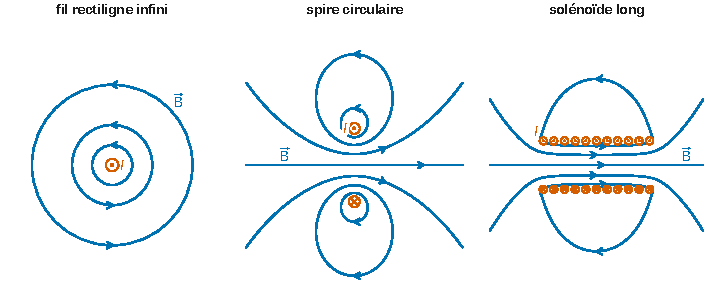
\includegraphics{figures/q2-lignes-fil-spire-solenoide.pdf}
\caption*{Figure 1 --- lignes de champ magnétique d'un fil infini vu en coupe,
d'une spire et d'un solénoïde vus en coupe par un plan contenant l'axe ;
⊙ courant vers le lecteur, ⊗ courant qui s'en éloigne}
\end{figure}

\begin{itemize}
\tightlist
\item
  \textbf{fil infini} : cercles centrés sur le fil, de plus en plus espacés ; pouce dans le sens de \(I\), les doigts donnent le sens de parcours ;
\item
  \textbf{spire circulaire} : lignes qui traversent le disque et se referment autour du conducteur ; au centre, \(\vec B\) suit l'axe, dans le sens du pouce quand les doigts suivent \(I\) ;
\item
  \textbf{solénoïde long} : lignes parallèles et serrées à l'intérieur (champ quasi uniforme), évasées et très espacées à l'extérieur.
\end{itemize}

\begin{methode}

Sur un dessin de lignes de champ, l'espacement des lignes traduit l'intensité du champ : resserrées là où \(B\) est fort, espacées là où il est faible. Indiquez-le explicitement.

\end{methode}

\begin{jury}

Rapport 2026 : « Beaucoup de candidats ne connaissent pas la définition d'une ligne de champ ; les tracés demandés sont souvent incompréhensibles, « brouillons » ou très approximatifs. » Donnez la définition en une phrase, puis des tracés propres, orientés, avec le sens de \(I\) sur chacun.

\end{jury}

\hypertarget{question-3}{%
\subsection{Question 3}\label{question-3}}

\begin{indication}{1}

Commencez par les invariances, puis les symétries, avant d'écrire le moindre théorème.

\end{indication}

\begin{indication}{2}

Un plan contenant le fil est plan de symétrie des courants. Que dire de la direction d'un pseudovecteur en un point de ce plan ? Choisissez ensuite un contour d'Ampère sur lequel \(B\) est constant.

\end{indication}

\hypertarget{solution-2}{%
\subsubsection{Solution}\label{solution-2}}

\emph{Invariances} : par translation selon \((Oz)\) et par rotation autour de \((Oz)\), donc \(\vec B\) ne dépend que de \(r\).

\emph{Symétries} : le plan \((M,\vec e_r,\vec e_z)\) est plan de symétrie de la distribution de courants. \(\vec B\), pseudovecteur, est perpendiculaire à ce plan : \(\vec B(M)=B(r)\vec e_\theta\).

\emph{Théorème d'Ampère} sur le cercle d'axe \((Oz)\) et de rayon \(r\), orienté par \(\vec e_\theta\) (cohérent avec le sens de \(I\) selon \(\vec e_z\)) :

\equationajustee{\oint\vec B\cdot\mathrm d\vec\ell=2\pi rB(r)=\mu_0I}

\equationajustee{\boxed{\vec B(M)=\frac{\mu_0I}{2\pi r}\,\vec e_\theta}}

\begin{jury}

Rapport 2026 : « L'utilisation du théorème d'Ampère suppose une étude soignée des symétries et invariances des sources du champ magnétique, à savoir les courants électriques. » L'adverbe « soigneusement » de l'énoncé appelle donc les trois temps (invariances, symétries des courants, théorème intégral). Sans l'argument de symétrie, on ne peut pas sortir \(B\) de l'intégrale.

\end{jury}

\hypertarget{question-4}{%
\subsection{Question 4}\label{question-4}}

\begin{indication}{1}

Exprimez \(\vec e_z\) dans la base \((\vec e_r,\vec e_\theta)\) à l'aide de la figure 3 : la composante sur \(\vec e_\theta\) est négative pour \(0<\theta<\pi\).

\end{indication}

\begin{indication}{2}

Pour retrouver \(M\), placez-vous au pôle Nord géographique : quelle valeur de \(\theta\) ? Quelle composante reste ?

\end{indication}

\hypertarget{solution-3}{%
\subsubsection{Solution}\label{solution-3}}

\(\vec e_z=\cos\theta\,\vec e_r-\sin\theta\,\vec e_\theta\), donc \(\vec M=-M\cos\theta\,\vec e_r+M\sin\theta\,\vec e_\theta\) et \(\vec M\cdot\vec e_r=-M\cos\theta\). En \(r=R_T\) :

\equationajustee{\vec B(P)=\frac{\mu_0}{4\pi R_T^3}\Big[-3M\cos\theta\,\vec e_r+M\cos\theta\,\vec e_r-M\sin\theta\,\vec e_\theta\Big]}

\equationajustee{\boxed{\begin{aligned}
B_r&=-\frac{\mu_0M\cos\theta}{2\pi R_T^3}\\
B_\theta&=-\frac{\mu_0M\sin\theta}{4\pi R_T^3}\\
B_\varphi&=0
\end{aligned}}}

Au pôle Nord géographique (\(\theta=0\)), \(\vec B=-\dfrac{\mu_0M}{2\pi R_T^3}\vec e_r\) est vertical et dirigé vers le centre de la Terre, de norme \(B_0\). Donc

\equationajustee{\begin{aligned}
M&=\frac{2\pi R_T^3B_0}{\mu_0}\\
&=\frac{(6{,}4\cdot10^6)^3\times6{,}0\cdot10^{-5}}{2\cdot10^{-7}}\\
&\approx262\cdot10^{18}\times3{,}0\cdot10^2\\
&\approx7{,}9\cdot10^{22}\ \mathrm{A\cdot m^2}.
\end{aligned}}

\begin{piege}

\(\vec M\) pointe vers le \textbf{sud} : le pôle Nord géographique est un pôle « sud » magnétique, où les lignes de champ entrent dans la Terre. \(M\) dans le tableau est une norme positive, ne la confondez pas avec la composante \(-M\).

\end{piege}

\begin{jury}

Rapport 2026 : « Peu de candidats savent faire une projection d'une relation vectorielle donnée. » La question a été « globalement mal traitée ». Écrivez explicitement \(\vec e_z\) dans la base sphérique avant de projeter.

\end{jury}

\hypertarget{question-5}{%
\subsection{Question 5}\label{question-5}}

\begin{indication}{1}

Écrivez les unités SI de \(M\), de \(j\) et de \(R_N\), puis identifiez séparément les exposants de l'ampère et du mètre.

\end{indication}

\begin{indication}{2}

Pour commenter, comparez aussi le courant \textbf{total} qui circule dans le noyau.

\end{indication}

\hypertarget{solution-4}{%
\subsubsection{Solution}\label{solution-4}}

\(\mathrm{A\cdot m^2}=(\mathrm{A\cdot m^{-2}})^\alpha\,\mathrm m^\beta\) impose \(\alpha=1\) et \(\beta-2=2\) :

\equationajustee{\boxed{\begin{aligned}
\alpha&=1\\
\beta&=4
\end{aligned}}}

On a donc \(M=jR_N^4\), d'où

\equationajustee{\begin{aligned}
j&=\frac{7{,}9\cdot10^{22}}{(5{,}0\cdot10^5)^4}\\
&=\frac{7{,}9\cdot10^{22}}{6{,}25\cdot10^{22}}\\
&\approx1\ \mathrm{A\cdot m^{-2}}.
\end{aligned}}

Fil : \(j_{\text{fil}}=i/s=10^{-2}/10^{-6}=1\cdot10^4\ \mathrm{A\cdot m^{-2}}\).

\textbf{La densité de courant du noyau est \(10^4\) fois plus faible que celle d'un modeste fil de laboratoire.} C'est l'immense extension du noyau qui fait la valeur de \(M\) : le courant total à travers une section vaut \(jR_N^2\sim10^{11}\) à \(10^{12}\) A, et \(M\) varie comme \(R_N^4\).

\begin{methode}

Le résultat \(\beta=4\) se retrouve physiquement : un moment magnétique est un courant multiplié par une surface, \(M\sim I\,R^2\), et le courant vaut \(I\sim jR^2\).

\end{methode}

\begin{jury}

Rapport 2026 : « Le début de la question a été globalement bien traité, mais pas les applications numériques. » Sans calculatrice, isolez les puissances de dix (\(5^4=625\)) et donnez l'unité de \(j\).

\end{jury}

\hypertarget{question-6}{%
\subsection{Question 6}\label{question-6}}

\begin{indication}{1}

Utilisez les signes de \(B_r\) trouvés en Q4 dans chaque hémisphère pour orienter les lignes.

\end{indication}

\begin{indication}{2}

Pour la comparaison, cherchez ce qui brise la symétrie du dipôle dans la figure 2 : d'où vient le vent solaire ?

\end{indication}

\hypertarget{solution-5}{%
\subsubsection{Solution}\label{solution-5}}

\begin{figure}[H]
\centering
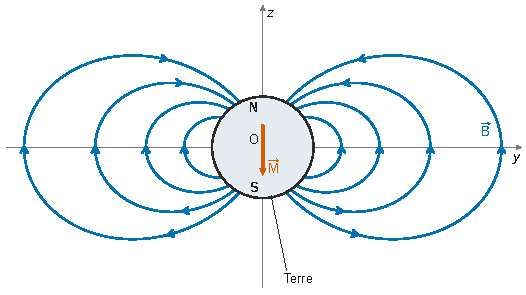
\includegraphics{figures/q6-lignes-dipole-terrestre.pdf}
\caption*{Figure 2 --- lignes de champ du dipôle géomagnétique dans le plan (yOz),
orientées du sud vers le nord à l'extérieur de la Terre}
\end{figure}

Dans le plan \((yOz)\), les lignes du dipôle sont des boucles fermées, symétriques par rapport à \((Oz)\) et au plan équatorial. Elles sont radiales près des pôles, parallèles à \((Oz)\) dans le plan équatorial, et s'éloignent d'autant plus de la Terre que leurs pieds sont proches de l'équateur.

\textbf{Orientation} : \(B_r<0\) dans l'hémisphère nord, \(B_r>0\) dans l'hémisphère sud. À l'extérieur de la Terre, \textbf{les lignes sortent de l'hémisphère sud et entrent dans l'hémisphère nord}, et \(\vec B\) est dirigé vers le nord (\(+\vec e_z\)) dans le plan équatorial.

Différences avec la figure 2 :

\begin{enumerate}
\def\labelenumi{\arabic{enumi}.}
\tightlist
\item
  \textbf{Dissymétrie jour/nuit} : côté Soleil, les lignes sont comprimées par le vent solaire ; côté nuit, elles sont étirées en une longue queue, quasi parallèle à l'axe Soleil-Terre, de part et d'autre de la couche de courant. Le dipôle, lui, est de révolution autour de \((Oz)\).
\item
  \textbf{Frontière et lignes ouvertes} : le champ terrestre est confiné par la magnétopause ; aux cornets polaires et dans la queue, des lignes ne se referment pas près de la Terre. Toutes les lignes du dipôle pur sont fermées et s'étendent sans limite.
\end{enumerate}

\begin{piege}

Vérifiez que les flèches de votre schéma sont cohérentes avec votre texte, \textbf{des deux côtés} de l'axe : dans le plan équatorial, le champ pointe vers le nord à droite comme à gauche.

\end{piege}

\begin{jury}

Rapport 2026 : « L'allure des lignes de champ a parfois été fantaisiste. Il fallait aussi faire attention au sens du dipôle magnétique. » Ici \(\vec M=-M\vec e_z\) pointe vers le sud : c'est lui qui fixe l'orientation des lignes.

\end{jury}

\hypertarget{question-7}{%
\subsection{Question 7}\label{question-7}}

\begin{indication}{1}

\(\theta\) est mesuré depuis l'axe \((Oz)\). Reprenez les composantes de Q4 avec \(r=d\).

\end{indication}

\begin{indication}{2}

Pour commenter, exprimez \(B(A)\) en fonction de \(B_0\) : quel facteur numérique ?

\end{indication}

\hypertarget{solution-6}{%
\subsubsection{Solution}\label{solution-6}}

\(\boxed{\theta=\pi/2}\). Avec \(r=d\) :

\equationajustee{\boxed{\begin{aligned}
B_r&=0\\
B_\theta&=-\frac{\mu_0M}{4\pi d^3}\\
B_\varphi&=0
\end{aligned}}}

À l'équateur, \(\vec e_\theta=-\vec e_z\), donc le champ est dirigé vers le nord :

\equationajustee{\vec B(A)=\frac{\mu_0M}{4\pi d^3}\vec e_z.}

\(B(A)=\dfrac{B_0}{2}\left(\dfrac{R_T}{d}\right)^3=\dfrac{6{,}0\cdot10^{-5}}{432}\approx1{,}4\cdot10^{-7}\) T. On retrouve la valeur de l'énoncé.

\textbf{Commentaire} : décroissance en \(1/r^3\) du champ dipolaire. À \(6R_T\), le champ est 430 fois plus faible qu'au pôle (\(6^3=216\), et un facteur 2 entre pôle et équateur). Il domine pourtant encore largement le champ quasi nul du vent solaire (quelques nT) : c'est bien une région sous contrôle du champ terrestre.

\begin{jury}

Rapport 2026 : « Question souvent mal traitée dans son ensemble et les commentaires simplistes. » Un commentaire utile est chiffré : facteur de décroissance par rapport au pôle, comparaison au champ du vent solaire, lien avec la position de la magnétopause.

\end{jury}

\hypertarget{question-8}{%
\subsection{Question 8}\label{question-8}}

\begin{indication}{1}

Partez du PFD avec la seule force \(q\vec v\wedge\vec B\) : que dire de la norme de la vitesse et de la composante \(v_z\) ?

\end{indication}

\begin{indication}{2}

Écrivez \(\vec v=R\dot\theta\,\vec e_\theta\) et \(\vec a=-R\dot\theta^2\vec e_r\) : la projection radiale donne \(\dot\theta\) \textbf{avec son signe}, donc le sens de rotation de chaque charge.

\end{indication}

\begin{indication}{3}

Pour le dessin, partez de la force au point d'entrée A : vers où pousse-t-elle le proton, et l'électron ?

\end{indication}

\hypertarget{solution-7}{%
\subsubsection{Solution}\label{solution-7}}

Le poids est négligeable devant la force magnétique. Avec \(\vec B=B\vec e_z\) :

\equationajustee{m\frac{\mathrm d\vec v}{\mathrm dt}=q\vec v\wedge\vec B.}

La puissance de la force est nulle, donc \(v\) est constante ; \(v_z\) est constante et nulle, donc le mouvement reste dans le plan \((xOy)\).

Mouvement circulaire de rayon \(R\), en base locale cylindrique centrée sur le centre de la trajectoire :

\equationajustee{\begin{aligned}
m\vec a&=-mR\dot\theta^2\,\vec e_r\\
q\vec v\wedge\vec B&=qR\dot\theta B\,(\vec e_\theta\wedge\vec e_z)=qR\dot\theta B\,\vec e_r
\end{aligned}}

L'égalité des deux donne

\equationajustee{\dot\theta=-\frac{qB}{m}}

\equationajustee{\boxed{R=\frac{mv}{\lvert q\rvert B}}}

Le \textbf{proton} (\(q>0\), \(\dot\theta<0\)) tourne dans le \textbf{sens horaire} vu depuis \(+\vec e_z\) (vu par le lecteur de la figure 5) ; l'\textbf{électron} tourne dans le \textbf{sens antihoraire}.

Dessin :

\begin{figure}[H]
\centering
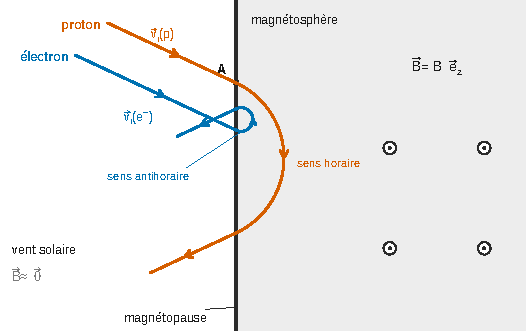
\includegraphics{figures/q8-trajectoires-magnetopause.pdf}
\caption*{Figure 3 --- trajectoires d'un proton, sens horaire, et d'un électron,
sens antihoraire, qui franchissent la magnétopause près de A ; rayons
non à l'échelle}
\end{figure}

Le proton, courbé vers le bas puis vers la gauche, ressort sous A ; l'électron, courbé vers le haut sur un arc minuscule, ressort au-dessus de son point d'entrée. Aucune ne pénètre au-delà de \(2R\) : la magnétosphère les \textbf{réfléchit}, c'est le rôle de bouclier.

Applications numériques (\(B=1{,}4\cdot10^{-7}\) T, \(v=7{,}0\cdot10^5\) m·s⁻¹) :

\equationajustee{\begin{aligned}
R_p&=\frac{2000\times9{,}1\cdot10^{-31}\times7{,}0\cdot10^5}{1{,}6\cdot10^{-19}\times1{,}4\cdot10^{-7}}\approx6\cdot10^4\ \mathrm m\\
R_e&=\frac{R_p}{2000}\approx3\cdot10^1\ \mathrm m
\end{aligned}}

\textbf{Commentaire} : \(R\ll d\approx4\cdot10^7\) m, ce qui justifie l'hypothèse d'un champ uniforme à l'échelle de la trajectoire. La réflexion se fait dans une couche très mince. Les deux espèces tournent en sens opposés et dérivent en sens contraires le long de la magnétopause, ce qui crée une séparation de charges et un courant de surface.

\begin{methode}

Pour trouver le sens de rotation sans erreur, calculez \(q\vec v\wedge\vec B\) en un point précis (ici A). Ou utilisez la règle : une charge positive tourne dans le sens horaire quand \(\vec B\) pointe vers l'observateur.

\end{methode}

\begin{piege}

L'électron et le proton ont la même vitesse mais pas la même masse : rapport des rayons \(m_p/m_e=2000\), pas 1. Faites aussi figurer cette différence d'échelle sur le dessin.

\end{piege}

\begin{jury}

Rapport 2026 : « À nouveau des schémas faux ou peu rigoureux avec des confusions. Cette question faisait appel à des connaissances de PCSI souvent oubliées sur le mouvement de particules chargées dans un champ magnétique. » Le sens de rotation de chaque charge doit se lire sur le dessin et découler du calcul.

\end{jury}

\hypertarget{partie-ii-uxe5ngstruxf6m-rydberg-et-bohr}{%
\section{Partie II -- Ångström, Rydberg\ldots{} et Bohr}\label{partie-ii-uxe5ngstruxf6m-rydberg-et-bohr}}

On construit le modèle de Bohr (orbite circulaire, quantification du moment cinétique) pour retrouver la formule de Rydberg, puis on teste l'hypothèse d'une raie d'aurore due à l'hydrogène. Outils : mécanique du point en force centrale, énergie, premiers éléments de physique quantique.

\hypertarget{question-9}{%
\subsection{Question 9}\label{question-9}}

\begin{indication}{1}

La force de Coulomb est centrale : appliquez le théorème du moment cinétique en \(O\).

\end{indication}

\begin{indication}{2}

Un vecteur constant colinéaire à \(\vec e_z\) est orthogonal à \(\overrightarrow{OM}\) à tout instant. Pour l'uniformité, que vaut \(L_O\) sur un cercle ?

\end{indication}

\hypertarget{solution-8}{%
\subsubsection{Solution}\label{solution-8}}

La force de Coulomb est colinéaire à \(\overrightarrow{OM}\) :

\equationajustee{\vec F=-\frac{e^2}{4\pi\varepsilon_0r^2}\vec e_r.}

Le théorème du moment cinétique en \(O\) fixe donne

\equationajustee{\frac{\mathrm d\vec L_O}{\mathrm dt}=\overrightarrow{OM}\wedge\vec F=\vec 0.}

Donc \(\vec L_O=m_e\overrightarrow{OM}\wedge\vec v\) est constant.

Si la position et la vitesse initiales sont dans \((xOy)\), \(\vec L_O\) est colinéaire à \(\vec e_z\) pour tout \(t\). Or \(\overrightarrow{OM}\cdot\vec L_O=0\) (produit mixte avec un vecteur répété), donc \(z(t)=0\) : \textbf{le mouvement est plan}.

Sur l'orbite circulaire, \(L_O=m_er_n^2\dot\theta\) est constant avec \(r_n\) fixé, donc \(\dot\theta\) est constant et \(v=r_n\lvert\dot\theta\rvert\) aussi : \textbf{le mouvement est uniforme}. L'accélération, elle, n'est pas nulle : elle est centripète.

\begin{piege}

Plan ne veut pas dire uniforme : c'est la conservation de \(L_O\) \textbf{à rayon fixé} qui donne l'uniformité. Et uniforme ne veut pas dire accélération nulle : sur un cercle parcouru à vitesse constante, \(\vec a=-\frac{v^2}{r_n}\vec e_r\).

\end{piege}

\begin{jury}

Rapport 2026 : « Trop de candidats pensent qu'un mouvement plan est forcément uniforme. Pour d'autres, un mouvement uniforme est caractérisé par un vecteur accélération nul. » Question jugée « très classique, du niveau PCSI » : elle doit être traitée sans faute.

\end{jury}

\hypertarget{question-10}{%
\subsection{Question 10}\label{question-10}}

\begin{indication}{1}

Accélération d'un mouvement circulaire uniforme, puis PFD projeté sur \(\vec e_r\).

\end{indication}

\hypertarget{solution-9}{%
\subsubsection{Solution}\label{solution-9}}

\equationajustee{m_e\frac{v_n^2}{r_n}=\frac{e^2}{4\pi\varepsilon_0r_n^2}}

\equationajustee{\boxed{v_n=\sqrt{\frac{e^2}{4\pi\varepsilon_0m_er_n}}}}

\begin{jury}

Rapport 2026 : « Il était inutile ici de chercher des équations horaires du mouvement. » La projection radiale du PFD suffit.

\end{jury}

\hypertarget{question-11}{%
\subsection{Question 11}\label{question-11}}

\begin{indication}{1}

L'énergie potentielle coulombienne s'annule à l'infini ; utilisez \(v_n^2\) trouvé en Q10.

\end{indication}

\hypertarget{solution-10}{%
\subsubsection{Solution}\label{solution-10}}

\equationajustee{\begin{aligned}
E_c&=\frac{e^2}{8\pi\varepsilon_0r_n}\\
E_p&=-\frac{e^2}{4\pi\varepsilon_0r_n}
\end{aligned}}

\equationajustee{\boxed{E_n=E_c+E_p=-\frac{e^2}{8\pi\varepsilon_0r_n}}}

\begin{methode}

Pour une orbite circulaire en \(1/r^2\) (Kepler ou Coulomb attractif), on a toujours \(E_m=-E_c=E_p/2\) : c'est un contrôle immédiat.

\end{methode}

\begin{piege}

Le rapport 2026 met en garde contre les racines carrées de valeurs négatives : \(E_n<0\), donc on ne tire jamais \(v_n\) de \(E_n=\frac12m_ev_n^2\). C'est \(E_c\), positive, qui donne la vitesse.

\end{piege}

\hypertarget{question-12}{%
\subsection{Question 12}\label{question-12}}

\begin{indication}{1}

Combinez \(m_er_nv_n=n\hbar\) avec l'expression de \(v_n\) (élevez au carré pour éliminer la racine).

\end{indication}

\begin{indication}{2}

Pour les conséquences, pensez à ce qu'impliquent des niveaux discrets pour la lumière émise, et à l'existence d'un niveau le plus bas.

\end{indication}

\hypertarget{solution-11}{%
\subsubsection{Solution}\label{solution-11}}

On combine la quantification et Q10 :

\equationajustee{\begin{aligned}
m_e^2r_n^2v_n^2&=n^2\hbar^2\\
v_n^2&=\frac{e^2}{4\pi\varepsilon_0m_er_n}\\
\frac{m_ee^2r_n}{4\pi\varepsilon_0}&=n^2\hbar^2
\end{aligned}}

\equationajustee{\boxed{r_n=a_0n^2}}

avec

\equationajustee{\boxed{a_0=\frac{4\pi\varepsilon_0\hbar^2}{m_ee^2}}}

En reportant dans \(E_n\) :

\equationajustee{E_n=-\frac{e^2}{8\pi\varepsilon_0a_0n^2}=-\frac{E_0}{n^2}}

\equationajustee{\boxed{\begin{aligned}
E_0&=\frac{e^2}{8\pi\varepsilon_0a_0}\\
&=\frac{m_ee^4}{32\pi^2\varepsilon_0^2\hbar^2}
\end{aligned}}}

(numériquement \(a_0\approx53\) pm et \(E_0\approx13{,}6\) eV).

Conséquences :

\begin{itemize}
\tightlist
\item
  les énergies sont \textbf{quantifiées} : l'atome n'émet ou n'absorbe que des photons d'énergie \(E_p-E_n\), d'où un \textbf{spectre de raies} ;
\item
  il existe un \textbf{état fondamental} stable (\(n=1\), rayon \(a_0\)) : l'électron ne s'effondre pas sur le noyau, et \(E_0\) est l'énergie d'ionisation de l'atome dans l'état fondamental. Tous les états liés ont \(E_n<0\), et \(E_n\to0\) quand \(n\to\infty\).
\end{itemize}

\hypertarget{question-13}{%
\subsection{Question 13}\label{question-13}}

\begin{indication}{1}

Conservation de l'énergie lors de l'émission d'un photon, puis \(E=hc/\lambda\).

\end{indication}

\hypertarget{solution-12}{%
\subsubsection{Solution}\label{solution-12}}

\equationajustee{\begin{aligned}
\frac{hc}{\lambda_{p\to n}}&=E_p-E_n\\
&=E_0\left(\frac1{n^2}-\frac1{p^2}\right)
\end{aligned}}

donc

\equationajustee{\boxed{R_\infty=\frac{E_0}{hc}}\qquad(\approx1{,}1\cdot10^7\ \mathrm{m^{-1}}).}

\hypertarget{question-14}{%
\subsection{Question 14}\label{question-14}}

\begin{indication}{1}

Étudiez la monotonie de \(\lambda_{p\to2}\) en fonction de \(p\) : où se placent les raies \(p\geq5\) par rapport à 486,2 nm ?

\end{indication}

\begin{indication}{2}

Pour les défauts, confrontez le modèle à l'électromagnétisme classique d'une part, à l'inégalité de Heisenberg d'autre part. Pour \(\psi\), partez de la normalisation.

\end{indication}

\hypertarget{solution-13}{%
\subsubsection{Solution}\label{solution-13}}

\equationajustee{\frac1{\lambda_{p\to2}}=R_\infty\left(\frac14-\frac1{p^2}\right)}

croît avec \(p\) : les raies de Balmer sont 656,3 nm, 486,2 nm, puis toutes en dessous de 486,2 nm (434, 410\ldots{} jusqu'à 365 nm).

557,7 nm est strictement entre \(\lambda_{4\to2}\) et \(\lambda_{3\to2}\). Il faudrait un \(p\) non entier (\(p\approx3{,}4\)), ce qui est impossible ; les autres séries sont hors du visible. \textbf{La raie verte n'est pas due à l'hydrogène atomique} (elle est due à l'oxygène atomique).

Défauts du modèle de Bohr :

\begin{itemize}
\tightlist
\item
  il utilise des \textbf{trajectoires} (position et vitesse définies simultanément), ce que l'inégalité de Heisenberg interdit ; la quantification \(L_O=n\hbar\) est postulée ;
\item
  un électron accéléré devrait \textbf{rayonner} et s'effondrer sur le noyau : la stabilité des orbites est imposée sans justification. Le modèle ne s'étend pas non plus aux atomes à plusieurs électrons.
\end{itemize}

\(\psi(x,t)\) est la \textbf{fonction d'onde}, une amplitude de probabilité. C'est l'interprétation probabiliste de Born : \(\lvert\psi\rvert^2\mathrm dx\) est la probabilité de trouver la particule entre \(x\) et \(x+\mathrm dx\), avec \(\int\lvert\psi\rvert^2\mathrm dx=1\). Donc

\equationajustee{\boxed{[\psi]=\mathrm m^{-1/2}}}

\begin{piege}

C'est \(\lvert\psi\rvert^2\) qui est une densité de probabilité (en \(\mathrm m^{-1}\) à une dimension), pas \(\psi\). Et constater que 557,7 nm diffère des deux valeurs données ne suffit pas : il faut exclure \textbf{toutes} les raies de la série.

\end{piege}

\begin{jury}

Rapport 2026 : les candidats « n'ont pas toujours su exploiter les données du sujet (valeurs des longueurs d'onde) et conclure sur la pertinence du modèle de Bohr dans ce contexte. Les défauts du modèle sont très rarement abordés. La fonction d'onde n'est pas adimensionnée, et l'interprétation donnée par Max Born rarement citée correctement. » Trois points faciles : une conclusion nette sur la raie verte, deux défauts, l'interprétation de Born avec la dimension de \(\psi\).

\end{jury}

\hypertarget{partie-iii-ondes-de-gravituxe9-dans-un-fjord-norvuxe9gien}{%
\section{Partie III -- Ondes de gravité dans un fjord norvégien}\label{partie-iii-ondes-de-gravituxe9-dans-un-fjord-norvuxe9gien}}

On linéarise les équations de l'hydrodynamique parfaite autour du repos, on cherche des modes harmoniques confinés près de la surface, et les deux conditions à l'interface (pression, cinématique) fournissent la relation de dispersion. Outils : dynamique des fluides, notation complexe, équation différentielle linéaire d'ordre 2.

Le rapport 2026 note que, dans cette partie, « Beaucoup de candidats se sont ainsi attachés à retrouver coûte que coûte les expressions données dans le texte, quitte à renoncer à la rigueur attendue. » Les résultats sont donnés : seule la rigueur du chemin rapporte des points.

\hypertarget{question-15}{%
\subsection{Question 15}\label{question-15}}

\begin{indication}{1}

Comparez par ordres de grandeur le terme convectif et le terme visqueux de l'équation (1).

\end{indication}

\hypertarget{solution-14}{%
\subsubsection{Solution}\label{solution-14}}

\equationajustee{\begin{aligned}
\lVert\rho(\vec v\cdot\overrightarrow{\operatorname{grad}})\vec v\rVert&\sim\rho\frac{U^2}{L}&&\text{(convection)}\\
\lVert\eta\Delta\vec v\rVert&\sim\eta\frac{U}{L^2}&&\text{(\text{viscosité})}
\end{aligned}}

\equationajustee{\boxed{R_e=\frac{\rho UL}{\eta}}}

\(R_e\), sans dimension, compare le transport convectif de quantité de mouvement à son transport diffusif par viscosité. \(R_e\ll1\) : écoulement dominé par la viscosité, laminaire. \(R_e\gg1\) : inertie dominante ; l'écoulement devient turbulent au-delà d'un seuil qui dépend de la géométrie (de l'ordre de \(2\cdot10^3\) dans une conduite cylindrique).

\begin{piege}

Le terme à comparer au terme visqueux est le terme \textbf{convectif} \((\vec v\cdot\overrightarrow{\operatorname{grad}})\vec v\), non le terme instationnaire.

\end{piege}

\begin{jury}

Rapport 2026 : « La définition du nombre de Reynolds et son interprétation ne sont pas maîtrisées par beaucoup de candidats. » Il faut les deux : le rapport des termes de l'équation (1) et le sens physique (convection contre diffusion visqueuse).

\end{jury}

\hypertarget{question-16}{%
\subsection{Question 16}\label{question-16}}

\begin{indication}{1}

« Parfait » renvoie à la viscosité, pas à la compressibilité.

\end{indication}

\hypertarget{solution-15}{%
\subsubsection{Solution}\label{solution-15}}

Écoulement parfait : viscosité négligeable, on supprime \(\eta\Delta\vec v\). On obtient l'\textbf{équation d'Euler} :

\equationajustee{\boxed{\rho\left(\frac{\partial\vec v}{\partial t}+(\vec v\cdot\overrightarrow{\operatorname{grad}})\vec v\right)=\rho\vec g-\overrightarrow{\operatorname{grad}}\,P}}

\hypertarget{question-17}{%
\subsection{Question 17}\label{question-17}}

\begin{indication}{1}

Vitesse nulle partout : il ne reste que la statique des fluides. Choisissez la constante d'intégration à la surface.

\end{indication}

\hypertarget{solution-16}{%
\subsubsection{Solution}\label{solution-16}}

\(\vec v=\vec 0\) annule le membre de gauche. Avec \(\vec g=-g\vec e_z\) (axe \((Oz)\) ascendant) :

\equationajustee{\begin{aligned}
\overrightarrow{\operatorname{grad}}\,P_e&=\rho\vec g\\
\frac{\mathrm dP_e}{\mathrm dz}&=-\rho g
\end{aligned}}

Avec \(P_e(0)=P_0\) :

\equationajustee{\boxed{P_e(z)=P_0-\rho gz}}

L'eau occupe \(z<0\) : la pression y est supérieure à \(P_0\) et croît avec la profondeur.

\begin{piege}

L'axe \((Oz)\) est orienté vers le \textbf{haut} et l'eau est en \(z<0\). Écrire \(P_e=P_0+\rho gz\) donnerait une pression qui diminue en descendant. Contrôlez toujours le signe : la pression d'un liquide au repos augmente avec la profondeur.

\end{piege}

\begin{jury}

Rapport 2026 : « Question mal traitée, ou de façon peu rigoureuse. Il fallait faire attention au sens de l'axe vertical. »

\end{jury}

\hypertarget{question-18}{%
\subsection{Question 18}\label{question-18}}

\begin{indication}{1}

Décomposez \(P=P_e+p\) dans l'équation d'Euler linéarisée et utilisez Q17.

\end{indication}

\begin{indication}{2}

Avec la notation complexe, une dérivée temporelle devient une multiplication par \(j\omega\) et une dérivée en \(x\) une multiplication par \(-jk\). La dérivée en \(z\) reste une dérivée.

\end{indication}

\begin{indication}{3}

Éliminez \(\underline V_x\) et \(\underline V_z\) entre les deux projections de (2) et la condition \(\operatorname{div}\vec v=0\).

\end{indication}

\hypertarget{solution-17}{%
\subsubsection{Solution}\label{solution-17}}

\(\rho\dfrac{\partial\vec v}{\partial t}=\rho\vec g-\overrightarrow{\operatorname{grad}}\,P_e-\overrightarrow{\operatorname{grad}}\,p\) et \(\overrightarrow{\operatorname{grad}}\,P_e=\rho\vec g\) donnent

\equationajustee{\boxed{\rho\frac{\partial\vec v}{\partial t}=-\overrightarrow{\operatorname{grad}}\,p}\qquad(2)}

\emph{Justification des formes sinusoïdales} : les équations (2) et \(\operatorname{div}\vec v=0\) sont linéaires, à coefficients indépendants de \(x\) et de \(t\). Une perturbation quelconque est une superposition de Fourier d'ondes \(e^{j(\omega t-kx)}\) qui évoluent indépendamment : il suffit d'en étudier une, avec une dépendance en \(z\) libre.

Projections de (2) :

\equationajustee{\begin{aligned}
j\omega\rho\,\underline V_x&=jkf\\
j\omega\rho\,\underline V_z&=-f'
\end{aligned}}

Incompressibilité : \(\boxed{\operatorname{div}\vec v=0}\), soit \(-jk\underline V_x+\underline V_z'=0\).

On y reporte \(\underline V_x=\dfrac{k}{\omega\rho}f\) et \(\underline V_z'=\dfrac{j}{\omega\rho}f''\) :

\equationajustee{-\frac{jk^2}{\omega\rho}f+\frac{j}{\omega\rho}f''=0}

\equationajustee{\boxed{f''-k^2f=0}}

\begin{methode}

Contrôle de cohérence : l'équation finale en \(f\) doit être réelle, sans \(j\) résiduel. Si un \(j\) subsiste, une conversion de dérivée est fausse.

\end{methode}

\begin{jury}

Rapport 2026, sur Q18 à Q20 : « Le jury attendait des justifications soignées. De nombreux candidats n'hésitent pas à modifier leurs calculs au fur et à mesure de leur avancée pour arriver à la bonne formule. » Un résultat donné par l'énoncé et atteint par un calcul ajusté après coup ne rapporte rien ; mieux vaut signaler honnêtement un écart.

\end{jury}

\hypertarget{question-19}{%
\subsection{Question 19}\label{question-19}}

\begin{indication}{1}

Solution générale en exponentielles réelles ; l'eau occupe \(z<0\) sur une profondeur \(H\gg\lambda\).

\end{indication}

\begin{indication}{2}

Pour \(e^{ka}\), comparez \(a\) à \(\lambda=2\pi/k\). Pour \(A\), écrivez que la pression totale de l'eau en \(z=h\) vaut \(P_0\), en utilisant Q17.

\end{indication}

\begin{indication}{3}

Pour \(\psi\), reprenez la projection de (2) sur \(\vec e_z\) : \(\psi\) est lié à la dérivée de \(f\).

\end{indication}

\hypertarget{solution-18}{%
\subsubsection{Solution}\label{solution-18}}

\(f(z)=Ae^{kz}+A'e^{-kz}\). Pour \(z\to-\infty\) (fond très lointain), \(e^{-kz}\) diverge, donc \(A'=0\). En prenant \(h=a\cos(\omega t-kx)\) comme référence de phase (\(A\) réel) :

\equationajustee{\boxed{p(x,z,t)=Ae^{kz}\cos(\omega t-kx)}}

\(ka=2\pi a/\lambda\ll1\), donc \(\boxed{e^{ka}\approx1}\), et de même \(e^{kh}\approx1\) puisque \(\lvert h\rvert\le a\).

Continuité de la pression en \(z=h\), avec \(e^{kh}\approx1\) :

\equationajustee{\begin{aligned}
P_0-\rho gh+Ae^{kh}\cos(\omega t-kx)&=P_0\\
A\cos(\omega t-kx)&=\rho ga\cos(\omega t-kx)
\end{aligned}}

pour tous \(x\) et \(t\), d'où

\equationajustee{\boxed{A=a\rho g}}

Projection de (2) sur \(\vec e_z\) :

\equationajustee{\underline V_z=-\frac{f'(z)}{j\omega\rho}}

donc \(\underline v\cdot\vec e_z=-\dfrac{1}{j\omega\rho}\psi(z)e^{j(\omega t-kx)}\) avec

\equationajustee{\boxed{\psi(z)=a\rho gk\,e^{kz}}}

La perturbation est confinée sur une profondeur de l'ordre de \(\lambda/2\pi\) : le fond, à 1 300 m, ne joue aucun rôle.

\begin{piege}

La condition de pression porte sur la pression \textbf{totale} \(P_e+p\) à la surface \textbf{déformée} : c'est le terme \(-\rho gh\) qui fixe \(A\). Écrire \(p=0\) en \(z=0\) donnerait \(A=0\).

\end{piege}

\hypertarget{question-20}{%
\subsection{Question 20}\label{question-20}}

\begin{indication}{1}

Que signifie, pour les particules d'eau de la surface, que la surface libre soit une frontière que l'eau ne traverse pas ?

\end{indication}

\begin{indication}{2}

Égalez les deux expressions de la vitesse verticale en \(z\approx0\) ; multipliez par \(j\omega\) pour faire disparaître les \(j\).

\end{indication}

\hypertarget{solution-19}{%
\subsubsection{Solution}\label{solution-19}}

C'est la \textbf{condition cinématique} : la surface libre est une surface matérielle, que le fluide ne traverse pas. La vitesse verticale de l'eau à la surface est égale à la vitesse verticale de déplacement de la surface (à l'ordre linéaire, en \(z\approx0\)).

\equationajustee{\begin{aligned}
-\frac{a\rho gk}{j\omega\rho}&=j\omega a\\
-agk&=j^2\omega^2a\qquad\text{(\text{après} multiplication par }j\omega)\\
-agk&=-\omega^2a
\end{aligned}}

Donc \(\omega^2=gk\) :

\equationajustee{\boxed{\omega=(gk)^{1/2}}}

L'exposant vaut

\equationajustee{\boxed{\beta=\tfrac12}}

Homogénéité : \([gk]=\mathrm{m\cdot s^{-2}\cdot m^{-1}}=\mathrm s^{-2}\), et \([\omega]=\mathrm s^{-1}\). C'est une \textbf{relation de dispersion} ; elle n'est pas linéaire, le milieu est dispersif.

\hypertarget{question-21}{%
\subsection{Question 21}\label{question-21}}

\begin{indication}{1}

Rappelez \(v_\varphi=\omega/k\) et \(v_g=\mathrm d\omega/\mathrm dk\), puis dérivez \(\sqrt{gk}\) par rapport à \(k\).

\end{indication}

\hypertarget{solution-20}{%
\subsubsection{Solution}\label{solution-20}}

La vitesse de phase est celle des surfaces d'égale phase ; la vitesse de groupe est celle de l'enveloppe d'un paquet d'ondes (transport de l'énergie).

\equationajustee{\begin{aligned}
v_\varphi&=\frac{\omega}{k}=\sqrt{\frac gk}\\
v_g&=\frac{\mathrm d\omega}{\mathrm dk}=\frac12\sqrt{\frac gk}
\end{aligned}}

\equationajustee{\boxed{v_g=\frac{v_\varphi}2}}

Les grandes longueurs d'onde vont le plus vite. Dans le sillage du navire, les crêtes naissent à l'arrière d'un groupe, le traversent et disparaissent à l'avant.

\begin{methode}

Pour une relation \(\omega\propto k^\beta\), on a toujours \(v_g=\beta\,v_\varphi\) : \(\beta=1/2\) pour la houle en eau profonde, \(\beta=1\) pour une onde non dispersive.

\end{methode}

\hypertarget{chimie-probluxe8me-1-partie-i-synthuxe8se-du-resvuxe9ratrol}{%
\section{Chimie, problème 1, partie I -- Synthèse du resvératrol}\label{chimie-probluxe8me-1-partie-i-synthuxe8se-du-resvuxe9ratrol}}

Le document 1 donne le cycle catalytique du couplage de Heck entre un iodure d'aryle et un styrène, tous deux porteurs de groupes acétate. Il faut lire le cycle (espèces entrantes et sortantes, état du palladium), nommer les actes élémentaires, puis déprotéger les phénols. Outils : chimie organométallique du programme de PC, réactivité des esters.

\hypertarget{question-22}{%
\subsection{Question 22}\label{question-22}}

\begin{indication}{1}

Repérez les espèces qui \textbf{entrent} dans le cycle (flèches courbes entrantes) et celles qui en \textbf{sortent} ; le complexe de palladium n'apparaît pas dans le bilan.

\end{indication}

\hypertarget{solution-21}{%
\subsubsection{Solution}\label{solution-21}}

Entrent : l'éthanoate de 4-iodophényle, le 3,5-diacétoxystyrène et Et₃N. Sortent : le stilbène triacétylé (E) et \(\mathrm{Et_3NH^+} + \mathrm{I^-}\).

\equationajustee{\mathrm{AcO{-}C_6H_4{-}I}\ +\ \mathrm{CH_2{=}CH{-}C_6H_3(OAc)_2}\ +\ \mathrm{Et_3N}\ \xrightarrow{\ \mathrm{Pd(0)}\ }\ \mathrm{AcO{-}C_6H_4{-}CH{=}CH{-}C_6H_3(OAc)_2\ (E)}\ +\ \mathrm{Et_3NH^+}\ +\ \mathrm{I^-}}

\begin{piege}

Les phénols sont encore protégés : le produit du cycle est l'acétate de resvératrol, pas le resvératrol. N'oubliez pas la base, consommée de façon stœchiométrique : c'est elle qui permet d'équilibrer l'équation, que le rapport 2026 juge « pas toujours équilibrée ».

\end{piege}

\hypertarget{question-23}{%
\subsection{Question 23}\label{question-23}}

\begin{indication}{1}

Comptez les ligands anioniques portés par Pd après l'étape 1 (aryle et iodure, plus électronégatifs que le métal).

\end{indication}

\hypertarget{solution-22}{%
\subsubsection{Solution}\label{solution-22}}

Pd(0) a un n.o. nul. Après l'étape 1, \(\mathrm{Ar{-}Pd{-}I}\) porte deux ligands anioniques (\(\mathrm{Ar^-}\), \(\mathrm{I^-}\)) : n.o. \(=+\mathrm{II}\).

\equationajustee{\boxed{\Delta\,\text{n.o.(Pd)}=+2}}

\begin{methode}

Une addition oxydante augmente le n.o. du métal de 2 ; une élimination réductrice le diminue de 2. Le n.o. du palladium doit revenir à 0 à la fin d'un tour de cycle.

\end{methode}

\begin{jury}

Le rapport 2026 regrette ici « l'absence fréquente de justification » : le résultat \(+2\) doit être accompagné du décompte des ligands anioniques.

\end{jury}

\hypertarget{question-24}{%
\subsection{Question 24}\label{question-24}}

\begin{indication}{1}

Faites le bilan atomique de l'étape 4 : le complexe de gauche perd l'alcène produit. Que reste-t-il sur le palladium ?

\end{indication}

\hypertarget{solution-23}{%
\subsubsection{Solution}\label{solution-23}}

L'étape 4 libère l'alcène couplé ; il reste sur le palladium l'iode et l'hydrogène arraché au carbone β :

\equationajustee{\boxed{\mathbf A=\mathrm{H{-}Pd{-}I}\ \ \text{(hydrido(iodo)palladium(II))}}}

À l'étape 5, Et₃N lui retire HI et Pd(0) est régénéré.

\begin{jury}

Rapport 2026 : « L'atome d'hydrogène est souvent oublié et des structures non réalistes sont souvent proposées. » Le bilan atomique de l'étape 4 (et la consommation de HI à l'étape 5) impose l'hydrure sur le palladium.

\end{jury}

\hypertarget{question-25}{%
\subsection{Question 25}\label{question-25}}

\begin{indication}{1}

Cinq noms d'actes élémentaires du cours : suivez le n.o. du palladium et le nombre de ligands d'une étape à l'autre.

\end{indication}

\begin{indication}{2}

Étape 3 : le groupe aryle passe du métal à l'alcène. Étape 5 : le n.o. du palladium redescend à 0.

\end{indication}

\hypertarget{solution-24}{%
\subsubsection{Solution}\label{solution-24}}

\begin{itemize}
\tightlist
\item
  Étape 1 : \textbf{addition oxydante} (Pd(0) → Pd(II)).
\item
  Étape 2 : \textbf{coordination} de l'alcène (complexe π).
\item
  Étape 3 : \textbf{insertion migratoire} 1,2 (syn) de l'alcène dans la liaison Pd--Ar.
\item
  Étape 4 : \textbf{β-élimination} d'hydrure (syn), qui libère le produit.
\item
  Étape 5 : \textbf{élimination réductrice} de HI (Pd(II) → Pd(0)), assistée par la base Et₃N.
\end{itemize}

\begin{methode}

La stéréosélectivité E s'explique par ces actes. L'insertion et l'élimination sont toutes deux syn. Entre les deux, une rotation autour de la liaison C--C place un H en syn du palladium. La conformation la moins encombrée, avec les deux aryles anti, conduit à l'alcène E.

\end{methode}

\begin{jury}

Rapport 2026 : « Les candidats proposent parfois aléatoirement des noms d'actes élémentaires et ce, en utilisant un vocabulaire approximatif. » Chaque nom se justifie par la variation du n.o. du métal et du nombre de ligands : c'est ce suivi qui évite les noms au hasard.

\end{jury}

\hypertarget{question-26}{%
\subsection{Question 26}\label{question-26}}

\begin{indication}{1}

Les OH sont masqués sous forme d'esters : quelle réaction coupe un ester de façon totale ?

\end{indication}

\begin{indication}{2}

En milieu basique, sous quelle forme se trouve un phénol ? Pensez au traitement final et à la quantité de base.

\end{indication}

\hypertarget{solution-25}{%
\subsubsection{Solution}\label{solution-25}}

\textbf{Conditions} : soude aqueuse ou hydroalcoolique en excès (au moins 6 équivalents : 3 pour les esters, 3 pour déprotoner les phénols libérés), puis acidification par \(\mathrm{H_3O^+}\). Alternative douce : \(\mathrm{K_2CO_3}\) dans le méthanol (transestérification). Réaction : \textbf{saponification}.

Mécanisme, pour chaque \(\mathrm{ArO{-}CO{-}CH_3}\) :

\begin{enumerate}
\def\labelenumi{\arabic{enumi}.}
\tightlist
\item
  \textbf{addition nucléophile} de \(\mathrm{HO^-}\) sur le carbone du carbonyle, qui donne l'intermédiaire tétraédrique \(\mathrm{ArO{-}C(O^-)(OH){-}CH_3}\) ;
\item
  \textbf{élimination} : C=O se reforme et expulse \(\mathrm{ArO^-}\), bon groupe partant (anion stabilisé par conjugaison avec le cycle) ; on obtient \(\mathrm{CH_3COOH}\) ;
\item
  \textbf{réaction acide-base totale} : \(\mathrm{CH_3COOH}\) est déprotoné en \(\mathrm{CH_3COO^-}\), ce qui rend la réaction totale ; les phénols restent sous forme de phénolates ;
\item
  \textbf{acidification} : \(\mathrm{ArO^-} + \mathrm{H_3O^+} \to \mathrm{ArOH} + \mathrm{H_2O}\). On isole le resvératrol.
\end{enumerate}

\begin{piege}

L'hydrolyse acide est un équilibre, lent et incomplet. Sans acidification finale, on n'isole pas le resvératrol mais son sel (le triphénolate).

\end{piege}

\begin{jury}

Rapport 2026 : « La saponification apparaît dans une fraction très faible de copies. Le mécanisme n'est pas souvent connu et son écriture manque de rigueur. » La question demande trois choses : les conditions opératoires (souvent omises selon le jury), le nom de la réaction et le mécanisme.

\end{jury}

\hypertarget{chimie-probluxe8me-1-partie-ii-dosage-des-polyphuxe9nols-par-la-muxe9thode-de-folin-ciocalteu}{%
\section{Chimie, problème 1, partie II -- Dosage des polyphénols par la méthode de Folin-Ciocalteu}\label{chimie-probluxe8me-1-partie-ii-dosage-des-polyphuxe9nols-par-la-muxe9thode-de-folin-ciocalteu}}

Le dosage est indirect : les polyphénols réduisent un réactif incolore en un mélange bleu dont on mesure l'absorbance. On en déduit une concentration en « équivalent acide gallique » à l'aide d'une droite d'étalonnage. Outils : dilutions, spectrophotométrie, loi de Beer-Lambert.

\hypertarget{question-27}{%
\subsection{Question 27}\label{question-27}}

\begin{indication}{1}

Conservation de la quantité de matière lors d'une dilution ; facteur de dilution 10.

\end{indication}

\hypertarget{solution-26}{%
\subsubsection{Solution}\label{solution-26}}

\(C_{\text{vin}}V_0=\dfrac{C_{\text{vin}}}{10}\times10{,}0\) mL, d'où

\equationajustee{\boxed{V_0=1{,}0\ \text{mL}}}

prélevé à la \textbf{pipette jaugée} de 1,00 mL, puis introduit dans une \textbf{fiole jaugée} de 10,0 mL complétée au trait de jauge avec de l'eau distillée et homogénéisée.

\begin{methode}

Dans un protocole de dosage, la verrerie fait partie de la réponse : pipette jaugée pour le prélèvement, fiole jaugée pour le volume final. Une éprouvette graduée n'est pas assez précise.

\end{methode}

\begin{piege}

Un volume à prélever supérieur au volume de la fiole (10,0 mL) signale une erreur de raisonnement. Le rapport 2026 relève que beaucoup de candidats qui l'ont obtenu n'ont pas douté de leur résultat : contrôlez toujours la cohérence.

\end{piege}

\hypertarget{question-28}{%
\subsection{Question 28}\label{question-28}}

\begin{indication}{1}

Deux arguments : la couleur de l'espèce qu'on dose (couleurs complémentaires), et ce qu'absorbe le vin lui-même (document 3).

\end{indication}

\hypertarget{solution-27}{%
\subsubsection{Solution}\label{solution-27}}

\begin{itemize}
\tightlist
\item
  Les polyphénols réduisent le réactif en oxydes \textbf{bleus} de W et Mo. Une espèce bleue absorbe dans le complémentaire, orange-rouge, jusqu'au proche infrarouge : elle absorbe fortement vers 700--800 nm (maximum des « bleus de molybdène » vers 760 nm).
\item
  D'après le document 3, le vin absorbe fortement dans l'UV (vers 280 nm) et un peu vers 520 nm (anthocyanes), mais \textbf{quasiment plus au-delà de 650--700 nm}.
\end{itemize}

À 760 nm, l'absorbance mesurée est donc due aux seuls oxydes bleus, dont la quantité est proportionnelle à celle des polyphénols. La couleur propre du vin n'interfère pas, et la sensibilité est bonne.

\begin{piege}

Ne choisissez pas la longueur d'onde « où le vin absorbe le plus » : on veut mesurer le produit de la réaction, pas la couleur de l'échantillon.

\end{piege}

\begin{jury}

Rapport 2026 : « Les candidats ont souvent confondu la longueur d'onde maximale d'absorption du complexe et la couleur réelle de l'échantillon analysée. » Le jury attendait le lien entre la couleur du complexe bleu et le spectre d'absorbance des autres composés du vin (document 3). Question souvent laissée de côté : elle rapporte pourtant avec deux arguments simples.

\end{jury}

\hypertarget{question-29}{%
\subsection{Question 29}\label{question-29}}

\begin{indication}{1}

Étalons et échantillon subissent exactement le même traitement : la droite donne directement la concentration de quelle solution ?

\end{indication}

\begin{indication}{2}

« Le plus précisément possible » : utilisez l'équation de la droite tracée (deux points bien choisis), pas seulement une lecture à l'œil. Remontez ensuite au vin avec le facteur de Q27.

\end{indication}

\hypertarget{solution-28}{%
\subsubsection{Solution}\label{solution-28}}

Les concentrations du document 4 sont celles des solutions de la gamme, traitées comme (S) (1,0 mL dans une fiole de 10,0 mL avec les mêmes réactifs). La droite donne donc directement \(C_S\).

La droite tracée passe par \((0\,;\,0{,}01)\) et \((0{,}30\,;\,1{,}01)\). Son coefficient directeur se calcule :

\equationajustee{a=\frac{1{,}01-0{,}01}{0{,}30-0}\approx3{,}3\ \mathrm{L\cdot g^{-1}}.}

La régression sur les dix points confirme \(A=3{,}33\,C+0{,}013\) (\(C\) en g·L⁻¹). Pour \(A=0{,}52\) :

\equationajustee{C_S=\frac{0{,}52-0{,}013}{3{,}33}\approx0{,}152\ \mathrm{g\cdot L^{-1}}}

On remonte au vin avec le facteur de dilution 10 de Q27 :

\equationajustee{\boxed{C_{\text{vin}}=10\,C_S\approx1{,}5\ \mathrm{g\cdot L^{-1}}\ \text{(\text{équivalent} acide gallique)}}}

soit environ 1 500 mg·L⁻¹, du même ordre que les vins du document 5.

\begin{piege}

Ne multipliez pas une seconde fois par 10 pour la fiole de dosage : étalons et échantillon y sont dilués de la même façon, ce facteur se compense. Le contrôle par ordre de grandeur (document 5) détecte immédiatement l'erreur : on trouverait 15 g·L⁻¹.

\end{piege}

\begin{jury}

D'après le rapport 2026, la lecture graphique est en général bien faite, mais l'énoncé (« le plus précisément possible ») invitait à calculer le coefficient directeur, et le facteur de dilution de Q27 a souvent été oublié : on rendait alors 0,15 g·L⁻¹ au lieu de 1,5 g·L⁻¹.

\end{jury}

\hypertarget{question-30}{%
\subsection{Question 30}\label{question-30}}

\begin{indication}{1}

Comparez au seuil du document 5, en tenant compte de l'incertitude de votre lecture.

\end{indication}

\hypertarget{solution-29}{%
\subsubsection{Solution}\label{solution-29}}

\(1{,}5\ \mathrm{g\cdot L^{-1}}<2\ \mathrm{g\cdot L^{-1}}\), avec une marge (0,5 g·L⁻¹) bien supérieure à l'incertitude de lecture (environ 0,1 g·L⁻¹ sur le vin) : \textbf{le vin n'est pas astringent} au sens du document 5. Sa teneur est comparable à celle des vins de Merlot et de Feteasca Neagra.

\begin{jury}

Question bien traitée selon le rapport 2026, qui relève une conclusion le plus souvent cohérente avec le résultat de Q29 : c'est ce lien explicite avec la valeur trouvée qui est attendu.

\end{jury}

\hypertarget{chimie-probluxe8me-2-partie-i-synthuxe8se-de-lacide-aspartique}{%
\section{Chimie, problème 2, partie I -- Synthèse de l'acide aspartique}\label{chimie-probluxe8me-2-partie-i-synthuxe8se-de-lacide-aspartique}}

Le document 6 décrit une synthèse malonique d'acide aminé. On prépare l'acide malonique, on le brome en α, on introduit l'azote, on protège les acides (esters) et l'amine (amide), on alkyle le carbone central, on coupe l'alcène par ozonolyse, puis on déprotège et on décarboxyle. Outils : substitution nucléophile, acidité en α des carbonyles, orbitales frontières, dérivés d'acides.

\hypertarget{question-31}{%
\subsection{Question 31}\label{question-31}}

\begin{indication}{1}

Deux réactifs, deux rôles : l'un est une base (comparez les \(\mathrm{p}K_a\) du tableau 3), l'autre un nucléophile.

\end{indication}

\begin{indication}{2}

Le carbone électrophile est primaire et porte un bon groupe partant : quel mécanisme ?

\end{indication}

\hypertarget{solution-30}{%
\subsubsection{Solution}\label{solution-30}}

\begin{enumerate}
\def\labelenumi{\arabic{enumi}.}
\tightlist
\item
  \textbf{Acide-base} : \(\mathrm{ClCH_2COOH} + \mathrm{HCO_3^-} \to \mathrm{ClCH_2COO^-} + \mathrm{CO_2} + \mathrm{H_2O}\), avec \(K=10^{6{,}4-5}\approx25\). Le carboxylate formé ne protone plus \(\mathrm{CN^-}\) en HCN, toxique et non nucléophile.
\item
  \textbf{\(S_N2\)} : le carbone de \(\mathrm{CN^-}\) attaque le \(\mathrm{CH_2}\) porteur du chlore à l'opposé de la liaison C--Cl ; la liaison C--C se forme pendant que C--Cl se rompt (état de transition unique), et \(\mathrm{Cl^-}\) part.
\end{enumerate}

\equationajustee{\boxed{\mathbf B=\mathrm{N{\equiv}C{-}CH_2{-}COO^-\,Na^+}\ \text{(\text{cyanoéthanoate} de sodium)}}}

L'étape 2 hydrolyse le nitrile en milieu acide et conduit à l'acide malonique C.

\begin{piege}

L'inversion de Walden n'a pas de conséquence ici : le carbone attaqué porte deux H et n'est pas stéréogène. Inutile de la développer.

\end{piege}

\begin{jury}

Rapport 2026 : « Cette question a été très peu abordée et les réponses correctes ont été encore plus rares. » C'est pourtant une \(S_N2\) de cours, précédée d'une réaction acide-base : les deux rôles (NaHCO₃ base, KCN nucléophile) suffisent à la débloquer.

\end{jury}

\hypertarget{question-32}{%
\subsection{Question 32}\label{question-32}}

\begin{indication}{1}

L'énol dérive de C par déplacement d'un H du carbone central vers l'oxygène du carbonyle. En milieu acide, par quoi commence-t-on ?

\end{indication}

\hypertarget{solution-31}{%
\subsubsection{Solution}\label{solution-31}}

Catalyse acide, sur une fonction COOH de \(\mathrm{HOOC{-}CH_2{-}COOH}\) :

\begin{enumerate}
\def\labelenumi{\arabic{enumi}.}
\tightlist
\item
  \textbf{protonation} de l'oxygène du carbonyle par \(\mathrm{H_3O^+}\) : on obtient un cation délocalisé sur le carbone et les deux oxygènes ;
\item
  \textbf{déprotonation du carbone α} par l'eau : le doublet C--H forme la liaison C=C, le doublet π de C=O⁺H revient sur l'oxygène, et \(\mathrm{H_3O^+}\) est régénéré.
\end{enumerate}

\equationajustee{\mathrm{HOOC{-}CH_2{-}C(=O)OH}\ \rightleftharpoons\ \mathrm{HOOC{-}CH{=}C(OH)_2}}

C'est la \textbf{tautomérie céto-énolique}, un équilibre très déplacé vers la forme carbonylée.

\begin{methode}

Une tautomérie est un équilibre entre isomères de constitution qui ne diffèrent que par la position d'un H et d'une double liaison. Le catalyseur (acide ou base) est régénéré : écrivez-le des deux côtés.

\end{methode}

\begin{piege}

En milieu basique, la déprotonation du carbone α donne l'\textbf{énolate}, pas l'énol demandé par le document 7 (et, avec un diacide, la base arrache d'abord les H des COOH). Écrivez un mécanisme en catalyse acide.

\end{piege}

\begin{jury}

Rapport 2026 : « Les candidats ont souvent proposé un mécanisme en milieu basique qui permettait d'expliquer la formation de l'énolate et non de l'énol. »

\end{jury}

\hypertarget{question-33}{%
\subsection{Question 33}\label{question-33}}

\begin{indication}{1}

Sous contrôle frontalier, l'électrophile interagit par sa BV avec une orbitale du nucléophile : laquelle ?

\end{indication}

\begin{indication}{2}

Comparez les coefficients de cette orbitale en \textbf{valeur absolue} sur tous les atomes, oxygènes compris.

\end{indication}

\hypertarget{solution-32}{%
\subsubsection{Solution}\label{solution-32}}

L'interaction dominante est \textbf{HO(énol, nucléophile) -- BV(\(\mathrm{Br_2}\), σ*)}. Elle est d'autant plus stabilisante que le recouvrement est grand, et son terme stabilisant varie comme le carré du coefficient de la HO sur l'atome attaqué.

\begin{longtable}[]{@{}
  >{\raggedright\arraybackslash}p{(\columnwidth - 14\tabcolsep) * \real{0.1250}}
  >{\raggedright\arraybackslash}p{(\columnwidth - 14\tabcolsep) * \real{0.1250}}
  >{\raggedright\arraybackslash}p{(\columnwidth - 14\tabcolsep) * \real{0.1250}}
  >{\raggedright\arraybackslash}p{(\columnwidth - 14\tabcolsep) * \real{0.1250}}
  >{\raggedright\arraybackslash}p{(\columnwidth - 14\tabcolsep) * \real{0.1250}}
  >{\raggedright\arraybackslash}p{(\columnwidth - 14\tabcolsep) * \real{0.1250}}
  >{\raggedright\arraybackslash}p{(\columnwidth - 14\tabcolsep) * \real{0.1250}}
  >{\raggedright\arraybackslash}p{(\columnwidth - 14\tabcolsep) * \real{0.1250}}@{}}
\toprule\noalign{}
\begin{minipage}[b]{\linewidth}\raggedright
Atome
\end{minipage} & \begin{minipage}[b]{\linewidth}\raggedright
1 (O)
\end{minipage} & \begin{minipage}[b]{\linewidth}\raggedright
2 (C)
\end{minipage} & \begin{minipage}[b]{\linewidth}\raggedright
3 (O)
\end{minipage} & \begin{minipage}[b]{\linewidth}\raggedright
4 (C)
\end{minipage} & \begin{minipage}[b]{\linewidth}\raggedright
5 (C)
\end{minipage} & \begin{minipage}[b]{\linewidth}\raggedright
6 (O)
\end{minipage} & \begin{minipage}[b]{\linewidth}\raggedright
7 (O)
\end{minipage} \\
\midrule\noalign{}
\endhead
\bottomrule\noalign{}
\endlastfoot
\(\lvert c_{\text{HO}}\rvert\) & 0,08 & 0,13 & 0,51 & \textbf{0,67} & 0,38 & 0,24 & 0,24 \\
\end{longtable}

Le coefficient maximal est sur l'\textbf{atome 4}, le carbone de la liaison C=C qui deviendra le carbone α (\(0{,}67^2\approx0{,}45\) contre \(0{,}26\) pour O3, le suivant). \(\mathrm{Br_2}\) est attaqué par C4 : le doublet π C4=C5 forme la liaison C4--Br et \(\mathrm{Br^-}\) part. Le cation formé, stabilisé par les oxygènes de C5, perd un proton et redonne la fonction acide. On obtient \(\mathrm{HOOC{-}CHBr{-}COOH}\) (D) : \textbf{bromation en α}.

\begin{piege}

C'est la HO du nucléophile qu'il faut lire, pas la BV : le tableau donne les deux. Et l'oxygène 3 a un coefficient non négligeable : il faut le citer et l'écarter explicitement.

\end{piege}

\begin{jury}

Le rapport 2026 relève de nombreuses conjectures sur la régiosélectivité ; les candidats qui ont exploité les coefficients des orbitales frontalières du document 7 ont en général conclu correctement. La justification attendue est donc chiffrée, à partir du tableau.

\end{jury}

\hypertarget{question-34}{%
\subsection{Question 34}\label{question-34}}

\begin{indication}{1}

Lisez attentivement les structures de F, G et J : quelles fonctions apparaissent, quelles fonctions disparaissent ? Regardez bien le réactif de l'étape 6 (que porte le carbonyle, en plus du chlore ?).

\end{indication}

\begin{indication}{2}

Pensez à ce qui gênerait l'étape 7 (EtONa, bromure d'allyle) et l'étape 8 (ozone) si les fonctions acide et amine étaient libres.

\end{indication}

\hypertarget{solution-33}{%
\subsubsection{Solution}\label{solution-33}}

\begin{itemize}
\tightlist
\item
  \textbf{Étape 5} : acidification, puis \textbf{estérification de Fischer} par l'éthanol. Les deux acides carboxyliques sont \textbf{protégés} en esters éthyliques. Sans cela, \(\mathrm{EtO^-}\) (étape 7) déprotonerait les COOH (\(\mathrm{p}K_a\approx5\)) au lieu du CH. Sous forme de diester, ce CH devient assez acide (\(\mathrm{p}K_a\approx13\)) pour être arraché par l'éthanolate, ce qui permet l'alkylation.
\item
  \textbf{Étape 6} : \textbf{N-acétylation} par le \textbf{chlorure d'acétyle} \(\mathrm{CH_3COCl}\) (NaHCO₃). L'amine est \textbf{protégée} sous forme d'\textbf{amide} (acétamide, \(\mathrm{NH{-}CO{-}CH_3}\)), peu nucléophile et peu basique. Libre, elle serait alkylée par le bromure d'allyle à l'étape 7 et oxydée par l'ozone à l'étape 8.
\item
  \textbf{Étape 9} : \textbf{déprotection} par hydrolyse basique (puis acidification). Les deux esters sont saponifiés, le COOH issu de l'ozonolyse est neutralisé, et l'acétamide est hydrolysé d'après la structure de J, qui porte \(\mathrm{NH_2}\). L'étape 10 décarboxyle à chaud le diacide gem (motif malonique) pour donner l'acide aspartique.
\end{itemize}

\begin{piege}

Le réactif de l'étape 6 est un chlorure d'\textbf{acyle} (\(\mathrm{CH_3{-}CO{-}Cl}\)), pas un chloroformiate (\(\mathrm{EtO{-}CO{-}Cl}\)) : G porte un groupe acétamide, pas un carbamate. Lisez toujours ce que porte le carbonyle d'un réactif dessiné en formule topologique.

\end{piege}

\begin{methode}

Pour justifier le rôle d'une étape de protection, nommez la fonction protégée, la forme protégée, et \textbf{l'étape ultérieure} que la fonction libre aurait perturbée.

\end{methode}

\begin{jury}

Rapport 2026 : « Il n'était pas suffisant de décrire le type de réaction réalisée, il fallait les envisager dans la globalité de la synthèse et en déduire leur raison d'être. » La séquence protection/déprotection est en général reconnue, mais les réponses manquent de précision sur les fonctions chimiques en jeu.

\end{jury}

\hypertarget{question-35}{%
\subsection{Question 35}\label{question-35}}

\begin{indication}{1}

Deux temps : des réactions acide-base (que deviennent les carboxylates et l'amine en milieu acide ?), puis le mécanisme de l'estérification de Fischer.

\end{indication}

\begin{indication}{2}

Fischer en cinq actes : activation électrophile, addition, prototropie, élimination, déprotonation.

\end{indication}

\hypertarget{solution-34}{%
\subsubsection{Solution}\label{solution-34}}

E \(=\mathrm{^-OOC{-}CH(NH_2){-}COO^-}\).

\begin{enumerate}
\def\labelenumi{\arabic{enumi}.}
\tightlist
\item
  \textbf{Acidification} : les \(\mathrm{COO^-}\) sont protonés en COOH et \(\mathrm{NH_2}\) en \(\mathrm{NH_3^+}\). L'ammonium n'est pas nucléophile, ce qui évite une amidation parasite.
\item
  \textbf{Estérification de Fischer}, pour chaque COOH :

  \begin{itemize}
  \item
    \begin{enumerate}
    \def\labelenumii{(\alph{enumii})}
    \tightlist
    \item
      protonation de l'O du carbonyle : le carbone devient plus électrophile ;
    \end{enumerate}
  \item
    \begin{enumerate}
    \def\labelenumii{(\alph{enumii})}
    \setcounter{enumii}{1}
    \tightlist
    \item
      addition nucléophile de l'oxygène de EtOH : on obtient l'intermédiaire tétraédrique \(\mathrm{R{-}C(OH)_2{-}O^+HEt}\) ;
    \end{enumerate}
  \item
    \begin{enumerate}
    \def\labelenumii{(\alph{enumii})}
    \setcounter{enumii}{2}
    \tightlist
    \item
      prototropie : \(\mathrm{H^+}\) passe sur un OH, qui devient \(\mathrm{{-}OH_2^+}\) ;
    \end{enumerate}
  \item
    \begin{enumerate}
    \def\labelenumii{(\alph{enumii})}
    \setcounter{enumii}{3}
    \tightlist
    \item
      élimination de \(\mathrm{H_2O}\) : on obtient l'ester protoné \(\mathrm{R{-}C(} = \mathrm{O^+H)OEt}\) ;
    \end{enumerate}
  \item
    \begin{enumerate}
    \def\labelenumii{(\alph{enumii})}
    \setcounter{enumii}{4}
    \tightlist
    \item
      déprotonation : on obtient l'ester, et \(\mathrm{H^+}\) est régénéré.
    \end{enumerate}
  \end{itemize}
\end{enumerate}

Après neutralisation de l'ammonium :

\equationajustee{\boxed{\mathbf F=\mathrm{EtO{-}CO{-}CH(NH_2){-}CO{-}OEt}}}

\begin{piege}

« 2 éq » d'éthanol, c'est la stœchiométrie exacte (un par fonction), pas un excès. L'estérification est un équilibre de constante voisine de 4 : en pratique, on la déplace avec l'éthanol en solvant ou en éliminant l'eau.

\end{piege}

\begin{jury}

Rapport 2026 : « Le mécanisme de la réaction d'estérification n'est pas maitrisé par un nombre important de candidats. Davantage de rigueur dans le formalisme des flèches courbes était attendu. » Chaque flèche part d'un doublet (liant ou non liant) et arrive sur un atome ou une liaison ; les charges doivent être portées à chaque étape.

\end{jury}

\hypertarget{question-36}{%
\subsection{Question 36}\label{question-36}}

\begin{indication}{1}

Classez les dérivés d'acide par réactivité vis-à-vis d'un nucléophile : où se place un chlorure d'acyle ?

\end{indication}

\begin{indication}{2}

L'acylation libère HCl : que ferait-il de l'amine ? Pourquoi une base faible plutôt que NaOH ou EtONa ? Comparez les \(\mathrm{p}K_a\) du tableau 3.

\end{indication}

\hypertarget{solution-35}{%
\subsubsection{Solution}\label{solution-35}}

\begin{itemize}
\tightlist
\item
  \textbf{\(\mathrm{CH_3COCl}\)} est l'agent d'acylation le plus réactif (\(\mathrm{Cl^-}\) excellent groupe partant, carbonyle très électrophile). L'acylation de l'amine (addition, puis élimination de \(\mathrm{Cl^-}\)) est rapide, totale et douce. L'amine, nucléophile le plus fort de F, est acylée sélectivement. Avec l'acide éthanoïque, on n'obtiendrait qu'une réaction acide-base.
\item
  \textbf{\(\mathrm{NaHCO_3}\)}, base faible (\(\mathrm{p}K_a=6{,}4\)) :

  \begin{itemize}
  \tightlist
  \item
    elle \textbf{neutralise HCl}, ce qui évite aussi un dégagement de chlorure d'hydrogène gazeux. Sinon, HCl protonerait l'amine restante en ammonium non nucléophile, et la conversion ne dépasserait pas 50 \% ;
  \item
    elle libère l'amine de son ammonium si F sort de l'étape 5 en milieu acide ;
  \item
    elle est \textbf{trop faible} pour saponifier les esters et pour déprotoner le CH central (\(\mathrm{p}K_a\approx13\gg6{,}4\)), ce qui évite toute réaction parasite sur le carbone. NaOH ou EtONa hydrolyseraient esters et chlorure d'acyle, ou formeraient l'énolate.
  \end{itemize}
\end{itemize}

\begin{methode}

Le choix d'une base se raisonne en \(\mathrm{p}K_a\) : assez forte pour capter l'acide formé (HCl), assez faible pour ne toucher à aucun autre site acide (\(\mathrm{p}K_a\) 13) ni aux fonctions électrophiles fragiles (esters).

\end{methode}

\begin{jury}

Rapport 2026 : « Les réponses à cette question sont souvent imprécises et incomplètes. L'argument selon lequel on souhaitait éviter la formation d'acide chlorhydrique gazeux apparaît tout de même assez fréquemment. » Cet argument ne suffit pas : il faut justifier les deux réactifs, chlorure d'acyle et base faible.

\end{jury}

\hypertarget{chimie-probluxe8me-2-partie-ii-cinuxe9tique-de-racuxe9misation-de-lacide-aspartique}{%
\section{Chimie, problème 2, partie II -- Cinétique de racémisation de l'acide aspartique}\label{chimie-probluxe8me-2-partie-ii-cinuxe9tique-de-racuxe9misation-de-lacide-aspartique}}

On modélise la racémisation post-mortem par deux réactions opposées d'ordre 1. On établit l'équation différentielle et sa linéarisation, puis on exploite des mesures à 65 °C. Outils : stéréochimie (CIP), cinétique formelle, régression linéaire, lecture graphique d'un logarithme.

\hypertarget{question-37}{%
\subsection{Question 37}\label{question-37}}

\begin{indication}{1}

Classez les quatre substituants par numéro atomique du premier atome, puis départagez les deux carbones au rang suivant.

\end{indication}

\begin{indication}{2}

Sur la figure 3, où est H (implicite) ? Lisez le sens de 1 → 2 → 3 avec H en arrière.

\end{indication}

\hypertarget{solution-36}{%
\subsubsection{Solution}\label{solution-36}}

Priorités : \(\mathrm{NH_2}\) (1) \textgreater{} COOH (2, carbone substitué par (O, O, O)) \textgreater{} \(\mathrm{CH_2COOH}\) (3, carbone substitué par (C, H, H)) \textgreater{} H (4).

Figure 3 : \(\mathrm C^*\) est au sommet bas du zigzag. \(\mathrm{CH_2}\) est en haut à gauche et COOH en haut à droite (dans le plan), \(\mathrm{NH_2}\) en coin plein vers le bas (vers l'observateur), et H implicite en arrière. H est en arrière ; on lit \(\mathrm{NH_2}\) (bas) → COOH (haut droite) → \(\mathrm{CH_2COOH}\) (haut gauche) : c'est le \textbf{sens antihoraire}.

\begin{figure}[H]
\centering
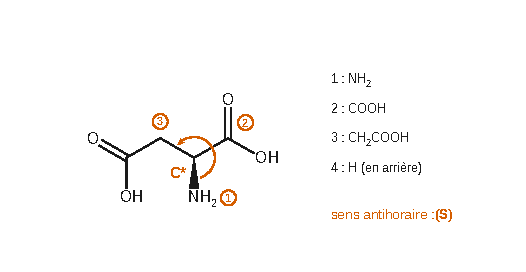
\includegraphics{figures/q37-cip-acide-l-aspartique.pdf}
\caption*{Figure 4 --- acide L-aspartique de la figure 3 annoté, priorités CIP 1 à
3 autour de C* et sens de rotation, H en arrière}
\end{figure}

\equationajustee{\boxed{\text{L-aspartique}=(S)}}

\begin{piege}

« L » (convention de Fischer) et « S » (CIP) sont deux systèmes différents : on ne déduit pas l'un de l'autre, on lit la figure. La L-cystéine, par exemple, est (R).

\end{piege}

\begin{jury}

Rapport 2026 : « Il convenait d'expliciter le sens de rotation et de faire le lien avec le descripteur stéréochimique. » Trois lignes suffisent : priorités justifiées, position de H, sens de rotation 1 → 2 → 3, donc S.

\end{jury}

\hypertarget{question-38}{%
\subsection{Question 38}\label{question-38}}

\begin{indication}{1}

Écrivez les vitesses des deux réactions opposées et faites le bilan de formation et de disparition de L.

\end{indication}

\hypertarget{solution-37}{%
\subsubsection{Solution}\label{solution-37}}

\equationajustee{\boxed{\frac{\mathrm d[\mathrm L]}{\mathrm dt}=-k_1[\mathrm L]+k_{-1}[\mathrm D]}}

\begin{piege}

Le rapport 2026 signale des erreurs de signe : L disparaît par la réaction directe (terme \(-k_1[\mathrm L]\)) et se forme par la réaction inverse (terme \(+k_{-1}[\mathrm D]\)).

\end{piege}

\hypertarget{question-39}{%
\subsection{Question 39}\label{question-39}}

\begin{indication}{1}

Définition : proportions des deux énantiomères.

\end{indication}

\hypertarget{solution-38}{%
\subsubsection{Solution}\label{solution-38}}

Un mélange \textbf{racémique} est un mélange équimolaire de deux énantiomères ; il est optiquement inactif. En fin de racémisation, \(\boxed{[\mathrm D]_\infty=[\mathrm L]_\infty}\).

\begin{piege}

« Mélange équimolaire de stéréoisomères » ne suffit pas : des diastéréoisomères en proportions égales ne forment pas un racémique. Le rapport 2026 insiste : il fallait préciser qu'il s'agit d'\textbf{énantiomères}.

\end{piege}

\hypertarget{question-40}{%
\subsection{Question 40}\label{question-40}}

\begin{indication}{1}

À l'état final, la concentration de L n'évolue plus : utilisez Q38 et Q39.

\end{indication}

\hypertarget{solution-39}{%
\subsubsection{Solution}\label{solution-39}}

À l'état final, \(\dfrac{\mathrm d[\mathrm L]}{\mathrm dt}=0\), donc

\equationajustee{k_1[\mathrm L]_\infty=k_{-1}[\mathrm D]_\infty.}

Avec Q39 (\([\mathrm L]_\infty=[\mathrm D]_\infty\neq0\)) :

\equationajustee{\boxed{k_1=k_{-1}=k}}

C'est cohérent avec \(K^\circ=k_1/k_{-1}=1\) pour deux énantiomères, qui ont la même enthalpie libre standard.

\hypertarget{question-41}{%
\subsection{Question 41}\label{question-41}}

\begin{indication}{1}

Conservation de la matière : que vaut \([\mathrm L]+[\mathrm D]\) à tout instant, en fonction de \([\mathrm L]_\infty\) ?

\end{indication}

\hypertarget{solution-40}{%
\subsubsection{Solution}\label{solution-40}}

La racémisation transforme L en D sans créer ni détruire d'acide aspartique : par \textbf{conservation de la matière}, la concentration totale est constante. Avec Q39 :

\equationajustee{\begin{aligned}
[\mathrm L]+[\mathrm D]&=[\mathrm L]_\infty+[\mathrm D]_\infty=2[\mathrm L]_\infty\\
[\mathrm D]&=2[\mathrm L]_\infty-[\mathrm L]
\end{aligned}}

On reporte dans Q38 avec \(k_1=k_{-1}=k\) :

\equationajustee{\frac{\mathrm d[\mathrm L]}{\mathrm dt}=-k[\mathrm L]+k\big(2[\mathrm L]_\infty-[\mathrm L]\big)}

\equationajustee{\boxed{\frac{\mathrm d[\mathrm L]}{\mathrm dt}+2k[\mathrm L]=2k[\mathrm L]_\infty}}

\begin{jury}

Rapport 2026 : « La conservation de la matière n'est que rarement mentionnée. » Le jury relève aussi des raisonnements confus chez ceux qui partent de l'équation donnée pour remonter le calcul. Écrivez le raisonnement dans le sens direct : bilan cinétique (Q38), conservation de la matière, substitution.

\end{jury}

\hypertarget{question-42}{%
\subsection{Question 42}\label{question-42}}

\begin{indication}{1}

D'après la relation admise, quelle fonction de \(r\) doit varier de façon affine avec \(t\) ? Quelle est la pente ?

\end{indication}

\begin{indication}{2}

Avant d'utiliser la droite du document 8, testez un point facile : pour \(r=0{,}333\), que vaut \(\frac{1-r}{1+r}\), et que vaut son logarithme népérien ? Comparez à l'ordonnée du point sur le graphe.

\end{indication}

\hypertarget{solution-41}{%
\subsubsection{Solution}\label{solution-41}}

Si l'ordre est 1, \(y=\ln\dfrac{1-r}{1+r}=y_0-2kt\) est affine en \(t\), avec \(y_0=\ln\dfrac{1-r_0}{1+r_0}\).

\begin{longtable}[]{@{}
  >{\raggedright\arraybackslash}p{(\columnwidth - 18\tabcolsep) * \real{0.1764}}
  >{\raggedright\arraybackslash}p{(\columnwidth - 18\tabcolsep) * \real{0.0882}}
  >{\raggedright\arraybackslash}p{(\columnwidth - 18\tabcolsep) * \real{0.0882}}
  >{\raggedright\arraybackslash}p{(\columnwidth - 18\tabcolsep) * \real{0.0882}}
  >{\raggedright\arraybackslash}p{(\columnwidth - 18\tabcolsep) * \real{0.0882}}
  >{\raggedright\arraybackslash}p{(\columnwidth - 18\tabcolsep) * \real{0.0882}}
  >{\raggedright\arraybackslash}p{(\columnwidth - 18\tabcolsep) * \real{0.0882}}
  >{\raggedright\arraybackslash}p{(\columnwidth - 18\tabcolsep) * \real{0.0882}}
  >{\raggedright\arraybackslash}p{(\columnwidth - 18\tabcolsep) * \real{0.0882}}
  >{\raggedright\arraybackslash}p{(\columnwidth - 18\tabcolsep) * \real{0.0882}}@{}}
\toprule\noalign{}
\begin{minipage}[b]{\linewidth}\raggedright
\(t\) (h)
\end{minipage} & \begin{minipage}[b]{\linewidth}\raggedright
24
\end{minipage} & \begin{minipage}[b]{\linewidth}\raggedright
48
\end{minipage} & \begin{minipage}[b]{\linewidth}\raggedright
108
\end{minipage} & \begin{minipage}[b]{\linewidth}\raggedright
240
\end{minipage} & \begin{minipage}[b]{\linewidth}\raggedright
432
\end{minipage} & \begin{minipage}[b]{\linewidth}\raggedright
672
\end{minipage} & \begin{minipage}[b]{\linewidth}\raggedright
864
\end{minipage} & \begin{minipage}[b]{\linewidth}\raggedright
936
\end{minipage} & \begin{minipage}[b]{\linewidth}\raggedright
1 272
\end{minipage} \\
\midrule\noalign{}
\endhead
\bottomrule\noalign{}
\endlastfoot
\(y=\ln\frac{1-r}{1+r}\) & −0,10 & −0,13 & −0,18 & −0,37 & −0,33 & −0,52 & −0,55 & −0,73 & −0,69 \\
\end{longtable}

\begin{figure}[H]
\centering
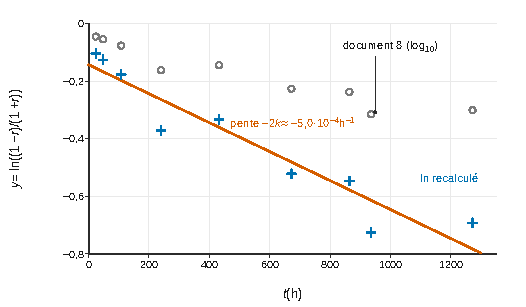
\includegraphics{figures/q42-linearisation-racemisation.pdf}
\caption*{Figure 5 --- y = ln((1 − r)/(1 + r)) en fonction de t, droite de
régression, et points du document 8 tracés en logarithme décimal}
\end{figure}

\emph{Validation du modèle affine.} Les points se répartissent autour d'une droite décroissante, sans courbure systématique (\(R\approx-0{,}95\)). La dispersion est réelle (deux inversions de \(r\)), mais typique de mesures sur échantillons biologiques.

\emph{Conclusion.} Le modèle affine étant validé, \textbf{les données sont compatibles avec un ordre partiel 1}. Régression, avec \(t\) en h :

\equationajustee{y\approx-5{,}0\cdot10^{-4}\,t-0{,}14}

La pente vaut \(-2k\), d'où

\equationajustee{\boxed{k_{65}\approx2{,}5\cdot10^{-4}\ \mathrm{h^{-1}}\approx7\cdot10^{-8}\ \mathrm{s^{-1}}}}

L'ordonnée à l'origine \(y_0\approx-0{,}14\) donne \(r_0\approx0{,}07\) : l'échantillon contenait déjà de l'acide D au départ.

\textbf{Erreur d'énoncé à signaler} : le graphe du document 8 est en \textbf{logarithme décimal} malgré son titre. Pour \(r=0{,}333\), on attend \(\ln\frac12\approx-0{,}69\), mais le point est placé à \(\log_{10}\frac12\approx-0{,}30\). La pente affichée, \(-2{,}18\cdot10^{-4}\) h⁻¹, vaut donc \(-2k/\ln10\). On retrouve

\equationajustee{k=\frac{2{,}3\times2{,}18\cdot10^{-4}}{2}\approx2{,}5\cdot10^{-4}\ \mathrm{h^{-1}},}

alors que la lecture naïve donnerait \(1{,}1\cdot10^{-4}\) h⁻¹.

\begin{jury}

Rapport 2026 : « Il convenait de valider le modèle affine et ensuite de conclure sur l'ordre 1. » La rigueur de cette détermination a manqué dans beaucoup de copies : d'abord l'argument sur l'alignement, ensuite seulement la conclusion sur l'ordre. Le rapport ne dit rien de l'erreur de logarithme du document 8 ; l'énoncé demande toutefois de signaler toute erreur repérée et d'expliquer l'initiative prise.

\end{jury}

\begin{piege}

Ne forcez pas la droite par l'origine en posant \(r_0=0\) : les données montrent \(r_0\neq0\). C'est la \textbf{pente} qui donne \(k\), l'ordonnée à l'origine ne fait que fixer \(r_0\).

\end{piege}

\hypertarget{question-43}{%
\subsection{Question 43}\label{question-43}}

\begin{indication}{1}

Traduisez « racémisé à 99 \% » en une valeur de \(r\), sachant que \(r_\infty=1\).

\end{indication}

\begin{indication}{2}

Isolez \(t\) dans la loi intégrée ; décomposez le logarithme pour utiliser les deux graphes de l'annexe 1.

\end{indication}

\hypertarget{solution-42}{%
\subsubsection{Solution}\label{solution-42}}

On prend \(r=0{,}99\). La loi intégrée donne

\equationajustee{t_{99}=\frac{y_0-\ln\dfrac{0{,}01}{1{,}99}}{2k}.}

Annexe 1 : \(\ln\dfrac{0{,}01}{1{,}99}=\ln(5{,}0\cdot10^{-3})\approx-5{,}3\), lu sur le graphe \(]0\,;0{,}1]\).

On peut aussi lire \(\ln0{,}01\approx-4{,}6\) et \(\ln1{,}99\approx0{,}7\) sur le graphe \(]0\,;2]\). Avec \(y_0\approx-0{,}14\) et \(2k\approx5{,}0\cdot10^{-4}\) h⁻¹ :

\equationajustee{\boxed{t_{99}\approx\frac{5{,}2}{5{,}0\cdot10^{-4}}\approx1\cdot10^4\ \text{h, soit environ 14 mois \text{à} }65\ ^\circ\mathrm C}}

Avec \(r_0=0\), on trouverait \(1{,}1\cdot10^4\) h, presque la même chose.

Si l'on comprend « racémisé à 99 \% » comme un excès énantiomérique résiduel de 1 \% (\(\frac{1-r}{1+r}=0{,}01\)), on trouve \(0{,}9\cdot10^4\) h : même ordre de grandeur.

En utilisant le graphe du document 8 sans correction, on trouverait \(2{,}4\cdot10^4\) h : c'est une erreur d'un facteur \(\ln10\) sur \(k\). À la température d'un sol, bien plus faible, la loi d'Arrhenius rend \(k\) beaucoup plus petit et la racémisation dure des milliers d'années : c'est ce qui permet la datation de restes anciens.

\begin{methode}

Pour lire un logarithme sur un graphe borné, factorisez : \(\ln(ab)=\ln a+\ln b\). On ramène ainsi n'importe quel nombre aux intervalles fournis.

\end{methode}

\begin{jury}

Rapport 2026 : « Les calculs conduisant à l'expression du temps ont souvent été confus. » Isolez d'abord \(t\) littéralement, puis seulement passez aux valeurs numériques.

\end{jury}

\hypertarget{bilan}{%
\section{Bilan}\label{bilan}}

\textbf{Méthodes à retenir}

\begin{itemize}
\tightlist
\item
  Calcul d'un champ magnétostatique : invariances, symétries (plan de symétrie des courants donc \(\vec B\) orthogonal), puis théorème d'Ampère. Projection d'un vecteur constant dans la base sphérique (\(\vec e_z=\cos\theta\,\vec e_r-\sin\theta\,\vec e_\theta\)).
\item
  Particule chargée dans \(\vec B\) uniforme : rayon \(mv/(\lvert q\rvert B)\). On obtient le sens de rotation par le signe de \(\dot\theta=-qB/m\), ou en calculant la force en un point.
\item
  Modèle de Bohr en trois lignes : PFD radial, quantification de \(L_O\), énergie \(-E_0/n^2\). Pour exclure une raie, raisonnez sur la monotonie de la série.
\item
  Houle linéaire : Euler linéarisée, modes \(f(z)e^{j(\omega t-kx)}\), incompressibilité, solution bornée \(e^{kz}\), condition dynamique (pression) puis condition cinématique ; on aboutit à \(\omega^2=gk\) et \(v_g=v_\varphi/2\).
\item
  Cycle catalytique : suivre le n.o. du métal et le bilan de chaque acte (addition oxydante, insertion, β-élimination, élimination réductrice).
\item
  Dosage par étalonnage : un traitement identique des étalons et de l'échantillon élimine les dilutions communes. On choisit la longueur d'onde là où seul le produit dosé absorbe.
\item
  Synthèse multi-étapes : pour chaque étape de protection, nommer la fonction protégée et l'étape qu'elle aurait gênée. On raisonne en \(\mathrm{p}K_a\) pour le choix des bases.
\item
  Réactions opposées d'ordre 1 : conservation de la matière, équilibre, linéarisation ; la pente donne \(k\), l'ordonnée fixe la condition initiale.
\end{itemize}

\textbf{Questions discriminantes en 2026} (rapport 2026) : les schémas (Q2, Q6, Q8), la projection en base sphérique (Q4), la statique orientée (Q17), l'intermédiaire de Heck et les actes élémentaires (Q24, Q25), la saponification (Q26), le choix de 760 nm (Q28) et, surtout, Q31, très peu abordée et rarement juste. En cinétique, Q41 (conservation de la matière) et Q43 (expression du temps) ont aussi séparé les copies.

\textbf{Prérequis à revoir} : base sphérique ; règle de la main droite ; notation complexe pour les ondes ; conditions aux limites à une interface fluide ; actes élémentaires organométalliques ; mécanismes de Fischer et de saponification ; règles CIP ; lecture critique d'un graphe (titre, échelle, unité).

\textbf{Questions classiques transposables} : Ampère pour un fil (tous concours) ; champ dipolaire et moment terrestre ; rayon cyclotron et confinement magnétique ; Bohr et Rydberg ; relation de dispersion de la houle (eau profonde, ou \(\omega^2=gk\tanh(kH)\) en profondeur finie) ; cycle de Heck et autres couplages au palladium (Suzuki) ; méthode de Folin-Ciocalteu et étalonnage spectrophotométrique ; synthèse malonique des acides aminés ; racémisation et datation des acides aminés.

\end{document}
